\documentclass[11pt, oneside]{article}

\usepackage[english]{babel}
\usepackage{geometry}  
\usepackage{graphicx}      
\usepackage{tabularx}      
\usepackage{amssymb}
\usepackage{amsmath}
\usepackage{booktabs}
\usepackage{hyperref}
\usepackage{achemso}
\usepackage{csquotes}
\usepackage{cleveref}
\usepackage{siunitx}
\usepackage{geometry}
\geometry{left=4cm, right=4cm}

\usepackage[dvipsnames]{xcolor}
\definecolor{tumblue}{rgb}{0,0.396078431372549,0.741176470588235}

\usepackage{xspace}
\usepackage{caption}
\usepackage{subcaption}
\usepackage{authblk} 

\usepackage{sectsty} 
\usepackage[acronym]{glossaries}
\usepackage[sort&compress,numbers,super]{natbib}

\sectionfont{\color{tumblue}\selectfont\sffamily}
\subsectionfont{\color{tumblue}\selectfont\sffamily}
\subsubsectionfont{\color{tumblue}\selectfont\sffamily}
\paragraphfont{\selectfont\sffamily}
\subparagraphfont{\color{gray}\selectfont\sffamily}


\renewcommand*{\Authfont}{\sf}
\renewcommand*{\Affilfont}{\sf}


\definecolor{halfgray}{gray}{0.55}
\renewcommand\labelitemi{\color{halfgray}$\bullet$} 

 
\usepackage{kpfonts}
\usepackage{biolinum}

\clubpenalty = 10000 
\widowpenalty = 10000 
\displaywidowpenalty = 10000


\usepackage{lipsum}
\usepackage[labelfont=bf]{caption}

\newacronym{llm}{LLM}{large language model}
\newacronym{ml}{ML}{machine learning}
\newacronym{agi}{AGI}{artificial general intelligence}
\newacronym{api}{API}{application programming interface}
\newacronym{mcq}{MCQ}{multiple-choice question}
\newacronym{rest}{REST}{Representational State Transfer}
\newacronym{orm}{ORM}{object relational mapping}
\newacronym{dai}{DAI}{daily allowed intake}
\newacronym{ghs}{GHS}{Globally Harmonized System of Classification and Labelling of Chemicals}
\newacronym{who}{WHO}{World Health Organization}
\newacronym{nmr}{NMR}{Nuclear Magnetic Resonance}
\newacronym{helm}{HELM}{Holistic Evaluation of Language Models}
\newacronym{smiles}{SMILES}{Simplified Molecular Input Line-Entry System}
\newacronym{pca}{PCA}{Principal Component Analysis}
\newacronym{iupac}{IUPAC}{International Union of Pure and Applied Chemistry}
\newacronym{json}{JSON}{JavaScript Object Notation}
\usepackage{credits}
\usepackage{orcidlink}
\usepackage{showyourwork}


\title{\textsf{Are large language models superhuman chemists?}}

%Conceptualization
%Data curation
%Formal analysis - Application of statistical, mathematical, computational, or other formal techniques to analyse or synthesize study data.
%Funding acquisition
%Investigation - Conducting a research and investigation process, specifically performing the experiments, or data/evidence collection.
%Methodology
%Project administration
%Resources
%Software
%Supervision
%Validation
%Visualization
%Writing -- original draft
%Writing -- review & editing


% Main contributors
\credit{Adrian~Mirza}{1,1,1,0,1,0,0,0,1,0,1,1,0,1}
\credit{Nawaf~Alampara}{1,1,1,0,1,0,0,0,1,0,1,0,0,1}
\credit{Sreekanth~Kunchapu}{1,1,0,0,1,0,0,0,0,0,1,0,0,1}
\credit{Martiño~Ríos-García}{1,1,1,0,1,0,0,0,1,0,1,0,0,1}


% Question contributors
\credit{Benedict~Emoekabu}{0,1,0,0,1,0,0,0,0,0,0,0,0,1}
\credit{Aswanth~Krishnan}{0,0,0,0,0,0,0,0,1,0,0,0,0,1}
\credit{Tanya~Gupta}{0,1,0,0,1,0,0,0,0,0,0,0,0,1}
\credit{Mara~Wilhelmi}{0,1,0,0,1,0,0,0,0,0,0,0,0,1}
\credit{Macjonathan~Okereke}{0,1,0,0,1,0,0,0,0,0,0,0,0,1}


% Question answerers
\credit{Mehrdad Asgari}{0,1,0,0,0,0,0,0,0,0,0,0,0,1}
\credit{Juliane Eberhardt}{0,1,0,0,0,0,0,0,0,0,0,0,0,1}
\credit{Amir~Mohammad~Elahi}{0,1,0,0,0,0,0,0,0,0,0,0,0,1}
\credit{Hani~M.~Elbeheiry~}{0,1,0,0,0,0,0,0,0,0,0,0,0,1}
\credit{María~Victoria~Gil}{0,1,0,0,1,0,0,0,0,0,0,0,0,1}
\credit{Christina Glaubitz}{0,1,0,0,0,0,0,0,0,0,0,0,0,1}
\credit{Maximilian Greiner}{0,1,0,0,0,0,0,0,0,0,0,0,0,1}
\credit{Caroline T. Holick}{0,1,0,0,0,0,0,0,0,0,0,0,0,1}
\credit{Tim Hoffmann}{0,1,0,0,0,0,0,0,0,0,0,0,0,1}
\credit{Abdelrahman~Ibrahim}{0,1,0,0,0,0,0,0,0,0,0,0,0,1}
\credit{Lea~C.~Klepsch}{0,1,0,0,0,0,0,0,0,0,0,0,0,1}
\credit{Yannik Köster}{0,1,0,0,0,0,0,0,0,0,0,0,0,1}
\credit{Fabian Alexander Kreth}{0,1,0,0,0,0,0,0,0,0,0,0,0,1}
\credit{Jakob~Meyer}{0,1,0,0,0,0,0,0,0,0,0,0,0,1}
\credit{Santiago~Miret}{0,1,0,0,0,0,0,0,0,0,0,0,0,1}
\credit{Jan Matthias Peschel}{0,1,0,0,0,0,0,0,0,0,0,0,0,1}
\credit{Michael Ringleb}{0,1,0,0,0,0,0,0,0,0,0,0,0,1}
\credit{Nicole Roesner}{0,1,0,0,0,0,0,0,0,0,0,0,0,1}
\credit{Johanna Schreiber}{0,1,0,0,0,0,0,0,0,0,0,0,0,1}
\credit{Ulrich~S.~Schubert}{0,0,0,1,0,0,0,0,0,0,0,0,0,1}
\credit{Leanne M. Stafast}{0,1,0,0,0,0,0,0,0,0,0,0,0,1}
\credit{Dinga Wonanke}{0,1,0,0,0,0,0,0,0,0,0,0,0,1}

% senior authors 
\credit{Michael~Pieler}{1,0,0,1,0,1,0,1,0,0,0,0,0,1}
\credit{Philippe~Schwaller}{1,1,0,1,1,1,0,0,0,1,0,0,0,1}
\credit{Kevin Maik Jablonka}{1,1,1,1,1,1,1,1,1,1,1,1,1,1}


\author[1,$\star$]{Adrian~Mirza~\orcidlink{0000-0003-4033-4235}}
\author[1,$\star$]{Nawaf~Alampara~\orcidlink{0009-0001-7697-7315}}
\author[1,$\star$]{Sreekanth~Kunchapu~\orcidlink{0009-0003-5752-0154}}
\author[1,x $\star$]{Martiño~Ríos-García~\orcidlink{0000-0003-1507-4048}}
\author[ ]{Benedict~Emoekabu}
\author[2]{Aswanth~Krishnan~\orcidlink{0009-0008-2703-5613}}
\author[3,4]{Tanya~Gupta~\orcidlink{0009-0001-9523-3290}}
\author[1]{Mara~Wilhelmi~\orcidlink{0009-0007-4392-5918}}
\author[1]{Macjonathan~Okereke~\orcidlink{0009-0007-1013-0502}}

\author[5]{Mehrdad~Asgari~\orcidlink{0000-0002-5427-1610}}
\author[6]{Juliane~Eberhardt~\orcidlink{0009-0000-3991-0704}}
\author[7]{Amir~Mohammad~Elahi~\orcidlink{0009-0001-5907-101X}}
\author[1]{Hani~M.~Elbeheiry~\orcidlink{0000-0002-5205-2852}}
\author[x]{María~Victoria~Gil~\orcidlink{0000-0003-4894-4660}}
\author[ ]{Christina~Glaubitz~\orcidlink{0000-0003-3412-0548}}
\author[1]{Maximilian~Greiner}
\author[1]{Caroline~T.~Holick~\orcidlink{0009-0000-1724-2725}}
\author[1]{Tim~Hoffmann~\orcidlink{0009-0004-0230-6115}}
\author[1]{Abdelrahman~Ibrahim~\orcidlink{0009-0003-1460-4710}}
\author[1]{Lea~C.~Klepsch~\orcidlink{0009-0009-3849-1670}}
\author[1]{Yannik~Köster~\orcidlink{0000-0002-9125-3067}}
\author[8, 9]{Fabian~Alexander~Kreth~\orcidlink{0000-0002-5968-8706}}
\author[1]{Jakob~Meyer}
\author[10]{Santiago~Miret~\orcidlink{0000-0002-4787-2757}}
\author[1]{Jan~Matthias~Peschel~\orcidlink{0009-0002-4787-2757}}
\author[1]{Michael~Ringleb~\orcidlink{0000-0002-7320-8529}}
\author[1, 11]{Nicole~Roesner~\orcidlink{0000-0002-5133-775X}}

\author[1, 10]{Johanna~Schreiber~\orcidlink{0009-0000-0991-8967}}
\author[1,8,11, 12]{Ulrich~S.~Schubert~\orcidlink{0000-0003-4978-4670}}
\author[1, 11]{Leanne~M.~Stafast~\orcidlink{0009-0008-5604-261X}}
\author[13]{Dinga~Wonanke~\orcidlink{0000-0002-9066-2715}}

% Senior authors
\author[14,15]{Michael~Pieler~\orcidlink{0000-0001-9186-7045}}
\author[3,4]{Philippe~Schwaller~\orcidlink{0000-0003-3046-6576}}
\author[1,8,11, 12, \Letter]{Kevin~Maik~Jablonka~\orcidlink{0000-0003-4894-4660}}



\affil[1]{Laboratory of Organic and Macromolecular Chemistry (IOMC), Friedrich Schiller University Jena, Humboldtstrasse 10, 07743 Jena, Germany}
\affil[2]{QpiVolta Technologies Pvt Ltd}
\affil[3]{Laboratory of Artificial Chemical Intelligence (LIAC), Institut des Sciences et Ing\'{e}nierie Chimiques, Ecole Polytechnique F\'{e}d\'{e}rale de Lausanne (EPFL), Lausanne, Switzerland}
\affil[4]{National Centre of Competence in Research (NCCR) Catalysis, Ecole Polytechnique F\'{e}d\'{e}rale de Lausanne (EPFL), Lausanne, Switzerland}
\affil[5]{Department of Chemical Engineering \& Biotechnology, University of Cambridge, Philippa Fawcett Drive, Cambridge CB3 0AS, United Kingdom}
\affil[6]{Macromolecular Chemistry, University of Bayreuth, 95447 Bayreuth, Germany}
\affil[7]{Laboratory of Molecular Simulation (LSMO), Institut des Sciences et Ing\'{e}nierie Chimiques, Ecole Polytechnique F\'{e}d\'{e}rale de Lausanne (EPFL), Sion, Switzerland}
\affil[8]{Center for Energy and Environmental Chemistry Jena (CEEC Jena), Friedrich Schiller University Jena, Philosophenweg 7a, 07743 Jena, Germany}
\affil[9]{Institute for Technical Chemistry and Environmental Chemistry (ITUC), Friedrich Schiller University Jena, Philosophenweg 7a, 07743 Jena, Germany}
\affil[10]{Intel Labs}
\affil[11]{Jena Center for Soft Matter (JCSM), Friedrich Schiller University Jena, Philosophenweg 7, 07743 Jena, Germany}
\affil[12]{Helmholtz Institute for Polymers in Energy Applications Jena (HIPOLE Jena), Lessingstrasse 12-14, 07743 Jena, Germany}
\affil[13]{Theoretical Chemistry, Technische Universität Dresden, Dresden 01062, Germany}
\affil[14]{OpenBioML.org}
\affil[15]{Stability.AI}

\affil[\Letter]{\texttt{mail@kjablonka.com}}
\affil[$\star$]{These authors contributed equally.}

\begin{document}
\maketitle

\clearpage
\begin{abstract}
    Large language models (LLMs) have gained widespread interest due to their ability to process human language. 
    Also, LLMs have shown promise in addressing the limited data problem in chemistry and are increasingly being harnessed to improve and extend existing workflows.

    However, we possess only a limited systematic understanding of the reasoning capabilities of LLMs, which would be required to improve models and mitigate potential harms. 
    Here, we introduce \enquote{\chembench,} an automated framework for evaluating the chemical knowledge and reasoning abilities of state-of-the-art LLMs against the expertise of chemists.

    We curated more than 2,800 question-answer pairs, evaluated leading open and closed-source LLMs, and found that, on average, the best models outperformed the chemists. 
    The models, however, struggle with some chemical reasoning tasks that are easy for the human experts and provide overconfident, misleading predictions, such as about chemicals' safety profiles. 
    Although LLMs demonstrate remarkable proficiency in chemical tasks, further research is critical to enhancing their safety and utility in chemical sciences.
\end{abstract}

\clearpage
\begin{refsection}
\section{Introduction}
\Glspl{llm} are \gls{ml} models trained on massive amounts of text to complete sentences. 
Aggressive scaling of these models has led to a rapid increase in their capabilities,\autocite{brown2020language,zhong2024benchmarking} with the leading models now being able to pass in some evaluations the United States Medical Licensing Examination.\autocite{kung2023performance} 
They also have been shown to design and autonomously perform chemical reactions when augmented with external tools such as web search and synthesis planners.\autocite{openai2024gpt4, Boiko_2023, bran2023chemcrow}
While some see \enquote{sparks of \gls{agi}} in them,\autocite{bubeck2023sparks} others consider them as \enquote{stochastic parrots}---i.e., systems that only regurgitate what they have been trained on.\autocite{bender2021dangers}
Nevertheless, the promise of these models is that they have shown the ability to solve a wide variety of tasks they have not been explicitly trained on.\autocite{bommasani2021opportunities, anderljung2023frontier, ai4science2023impact}
This has led to tremendous economic interest and investment in such generative models, with an expected market of more than \$1.3 trillion (almost \$30 billion for drug discovery applications) by 2032.\autocite{bloomberg}

Chemists and materials scientists have quickly caught on to the mounting attention given to \glspl{llm}, with some voices even suggesting that \enquote{the future of chemistry is language}.\autocite{White_2023}
This statement is motivated by a growing number of reports that use \glspl{llm} to predict properties of molecules or materials,\autocite{jablonka202314, jablonka2024leveraging, xie2024fine, liao2024words, zhang2024chemllm, zhong2024benchmarking}  optimize reactions\autocite{ramos2023bayesian, kristiadi2024sober}  generate materials,\autocite{rubungo2023llm, flam2023language, gruver2024fine} extract information,\autocite{Patiny_2023, Dagdelen_2024, Zheng_2024, lala2023paperqa, caufield2023structured, gupta2022discomat} or to even prototype systems that can autonomously perform reactions in the physical world based on commands provided in natural language.\autocite{bran2023chemcrow, Boiko_2023, darvish2024organa}

In addition, since a lot---if not most---of the information about chemistry is currently stored and communicated in text, there is a strong reason to believe that there is still a lot of untapped potential in \glspl{llm} for chemistry and materials science.\autocite{miret2024llms}
For instance, most insights in chemical research do not directly originate from data stored in databases but rather from the scientists and their ability to interpret data. 
Many of these insights are in the form of text in scientific publications. 
Thus, operating on such texts might be our best way of unlocking these insights and learning from them.
This might ultimately lead to general copilot systems for chemists that can provide answers to questions or even suggest new experiments based on vastly more information than a human could ever read.
Such a usage mode is, in particular, interesting in the face of recent advances in autonomous laboratories.\autocite{Boiko_2023, bran2023chemcrow, darvish2024organa, granda2018controlling, Angello_2022, coley2019robotic, Burger_2020, seifrid2022autonomous}


However, the rapid increase in capabilities of chemical \gls{ml} models led (even before the recent interest in \glspl{llm}) to concerns about the potential for dual use of these technologies, e.g., for the design of chemical weapons.\autocite{gopal2023releasing, ganguli2022red, Urbina_2022, campbell2023censoring, moulange2023towards, urbina2022teachable}
To some extent, this is not surprising as any technology that, for instance, is used to design non-toxic molecules can also be used inversely to predict toxic ones (even though the synthesis would still require access to controlled physical resources and facilities).
Still, it is essential to realize that such models' user base is wider than that of chemistry and materials science experts who critically reflect on every output such models produce. 
For example, many students frequently consult these tools---perhaps even to prepare chemical experiments.\autocite{Intelligent.com_2023}
This also applies to users from the general public, who might consider using \glspl{llm} to answer questions about the safety of chemicals.
Thus, for some users, misleading information---especially about safety-related aspects---might lead to harmful outcomes. 
However, even for experts, chemical understanding and reasoning capabilities are essential as they will determine the capabilities and limitations of their models in their work, e.g., in copilot systems for chemists.
Unfortunately, apart from anecdotal reports, there is little evidence on how \glspl{llm} perform compared to expert (human) chemists.

Thus, to better understand what \glspl{llm} can do for the chemical sciences and where they might be improved with further developments, evaluation frameworks are needed to allow us to measure progress and mitigate potential harms systematically.
For the development of \glspl{llm}, evaluation is currently primarily performed via standardized benchmark suites such as BigBench\autocite{srivastava2022beyond} or the LM Eval Harness.\autocite{eval-harness}
Among 204 tasks (such as linguistic puzzles), the former contains only two tasks classified as \enquote{chemistry related}, whereas the latter contains no specific chemistry tasks.
Due to the lack of widely accepted standard benchmarks, the developers of chemical language models\autocite{jablonka2024leveraging, guo2023large, ahmad2022chemberta2, Cai_2024, frey2023neural} frequently utilize language-interfaced\autocite{dinh2022lift} tabular datasets such as the ones reported in MoleculeNet,\autocite{wu2018moleculenet} Therapeutic Data Commons\autocite{huang2021therapeutics} or MatBench.\autocite{Dunn_2020}
In these cases, the models are evaluated on predicting very specific properties of molecules (e.g., solubility, toxicity, melting temperature or reactivity) or on predicting the outcome of specific chemical reactions.
This, however, only gives a very limited view of the general chemical capabilities of the models.

While some benchmarks based on university entrance exams\autocite{Zaki_2024, arora2023llms} or automatic text mining\autocite{song2023honeybee, wei2021chemistryqa, song-etal-2023-matsci} have been proposed, none of them have been widely accepted.
This is likely because they cannot automatically be used with black box (or tool-augmented) systems, do not cover a wide range of topics, or are not carefully validated by experts.
On top of that, the existing benchmarks are not designed to be used with models that support special treatment of molecules or equations and do not provide insights on how the models compare relative to experts.

In this work, we report a novel benchmarking framework  (\Cref{fig:overview_figure}), which we call \chembench, and use it to reveal limitations of current frontier models for use in the chemical sciences.
Our benchmark consists of \variable{output/total_number_of_questions.txt}\xspace question-answer pairs compiled from diverse sources (\variable{output/manually_generated.txt}\xspace manually generated, and \variable{output/automatically_generated.txt}\xspace automatically generated).  
Our corpus covers a large fraction of the topics taught in undergraduate and graduate chemistry curricula. It can be used to evaluate any system that can return text (i.e., including tool-augmented systems).

To contextualize the scores, we also surveyed \variable{output/number_experts.txt} experts in chemistry on a subset of the benchmark corpus to be able to compare the performance of current frontier models with (human) chemists of different specializations.
Our results indicate that current frontier models perform \enquote{superhuman} on some aspects of chemistry but, in many cases, including safety-related ones, might be very misleading.
We find that there are still numerous limitations for current models to overcome, such that they can be directly applied in autonomous systems for chemists.
Moreover, we conclude that carefully created broad benchmarks represent an important stepping stone for progress in this field.  %and underline the importance of careful evaluation of the capabilities of \glspl{llm} in the chemical sciences.

\section{Results and Discussion}

\begin{figure}
    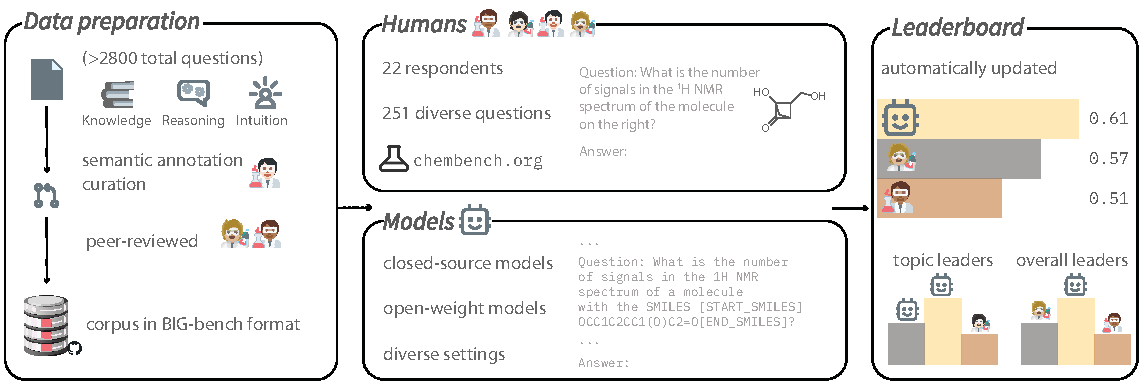
\includegraphics[width=\textwidth]{figures/overview_figure.pdf}
    \caption{\textbf{Overview of the \chembench framework.} The figure shows the different components of the \chembench framework. 
    The framework's foundation is the benchmark corpus that consists of many questions and answers that we manually or semi-automatically compiled from various sources.
    We then used this corpus to evaluate the performance of various models and tool-augmented systems using a custom framework. To provide a baseline, we built a web application that we used to survey experts in chemistry.
    The results of the evaluations are then compiled in publicly accessible leaderboards, which we propose as a foundation for evaluating future models.
    }
    \label{fig:overview_figure}
\end{figure}

\subsection{Benchmark corpus}

To compile our benchmark corpus, we utilized a broad list of sources (see \Cref{sec:curation}), ranging from university exams to semi-automatically generated questions based on curated subsets of data in chemical databases.
For quality assurance, all questions have been reviewed by at least one scientist in addition to the original curator and automated checks. 
Importantly, our large pool of questions encompasses a wide range of topics and question types. The topics range from general chemistry to more specialized fields such as inorganic, analytical or technical chemistry. 
We also classify the questions based on what techniques are required to answer them. Here, we distinguish between questions that require knowledge, reasoning, calculation, intuition or a combination of these.
Moreover, to allow for a more nuanced evaluation of the models capabilities, the questions are also classified by difficulty.

\begin{figure}[!htb]
    \centering
    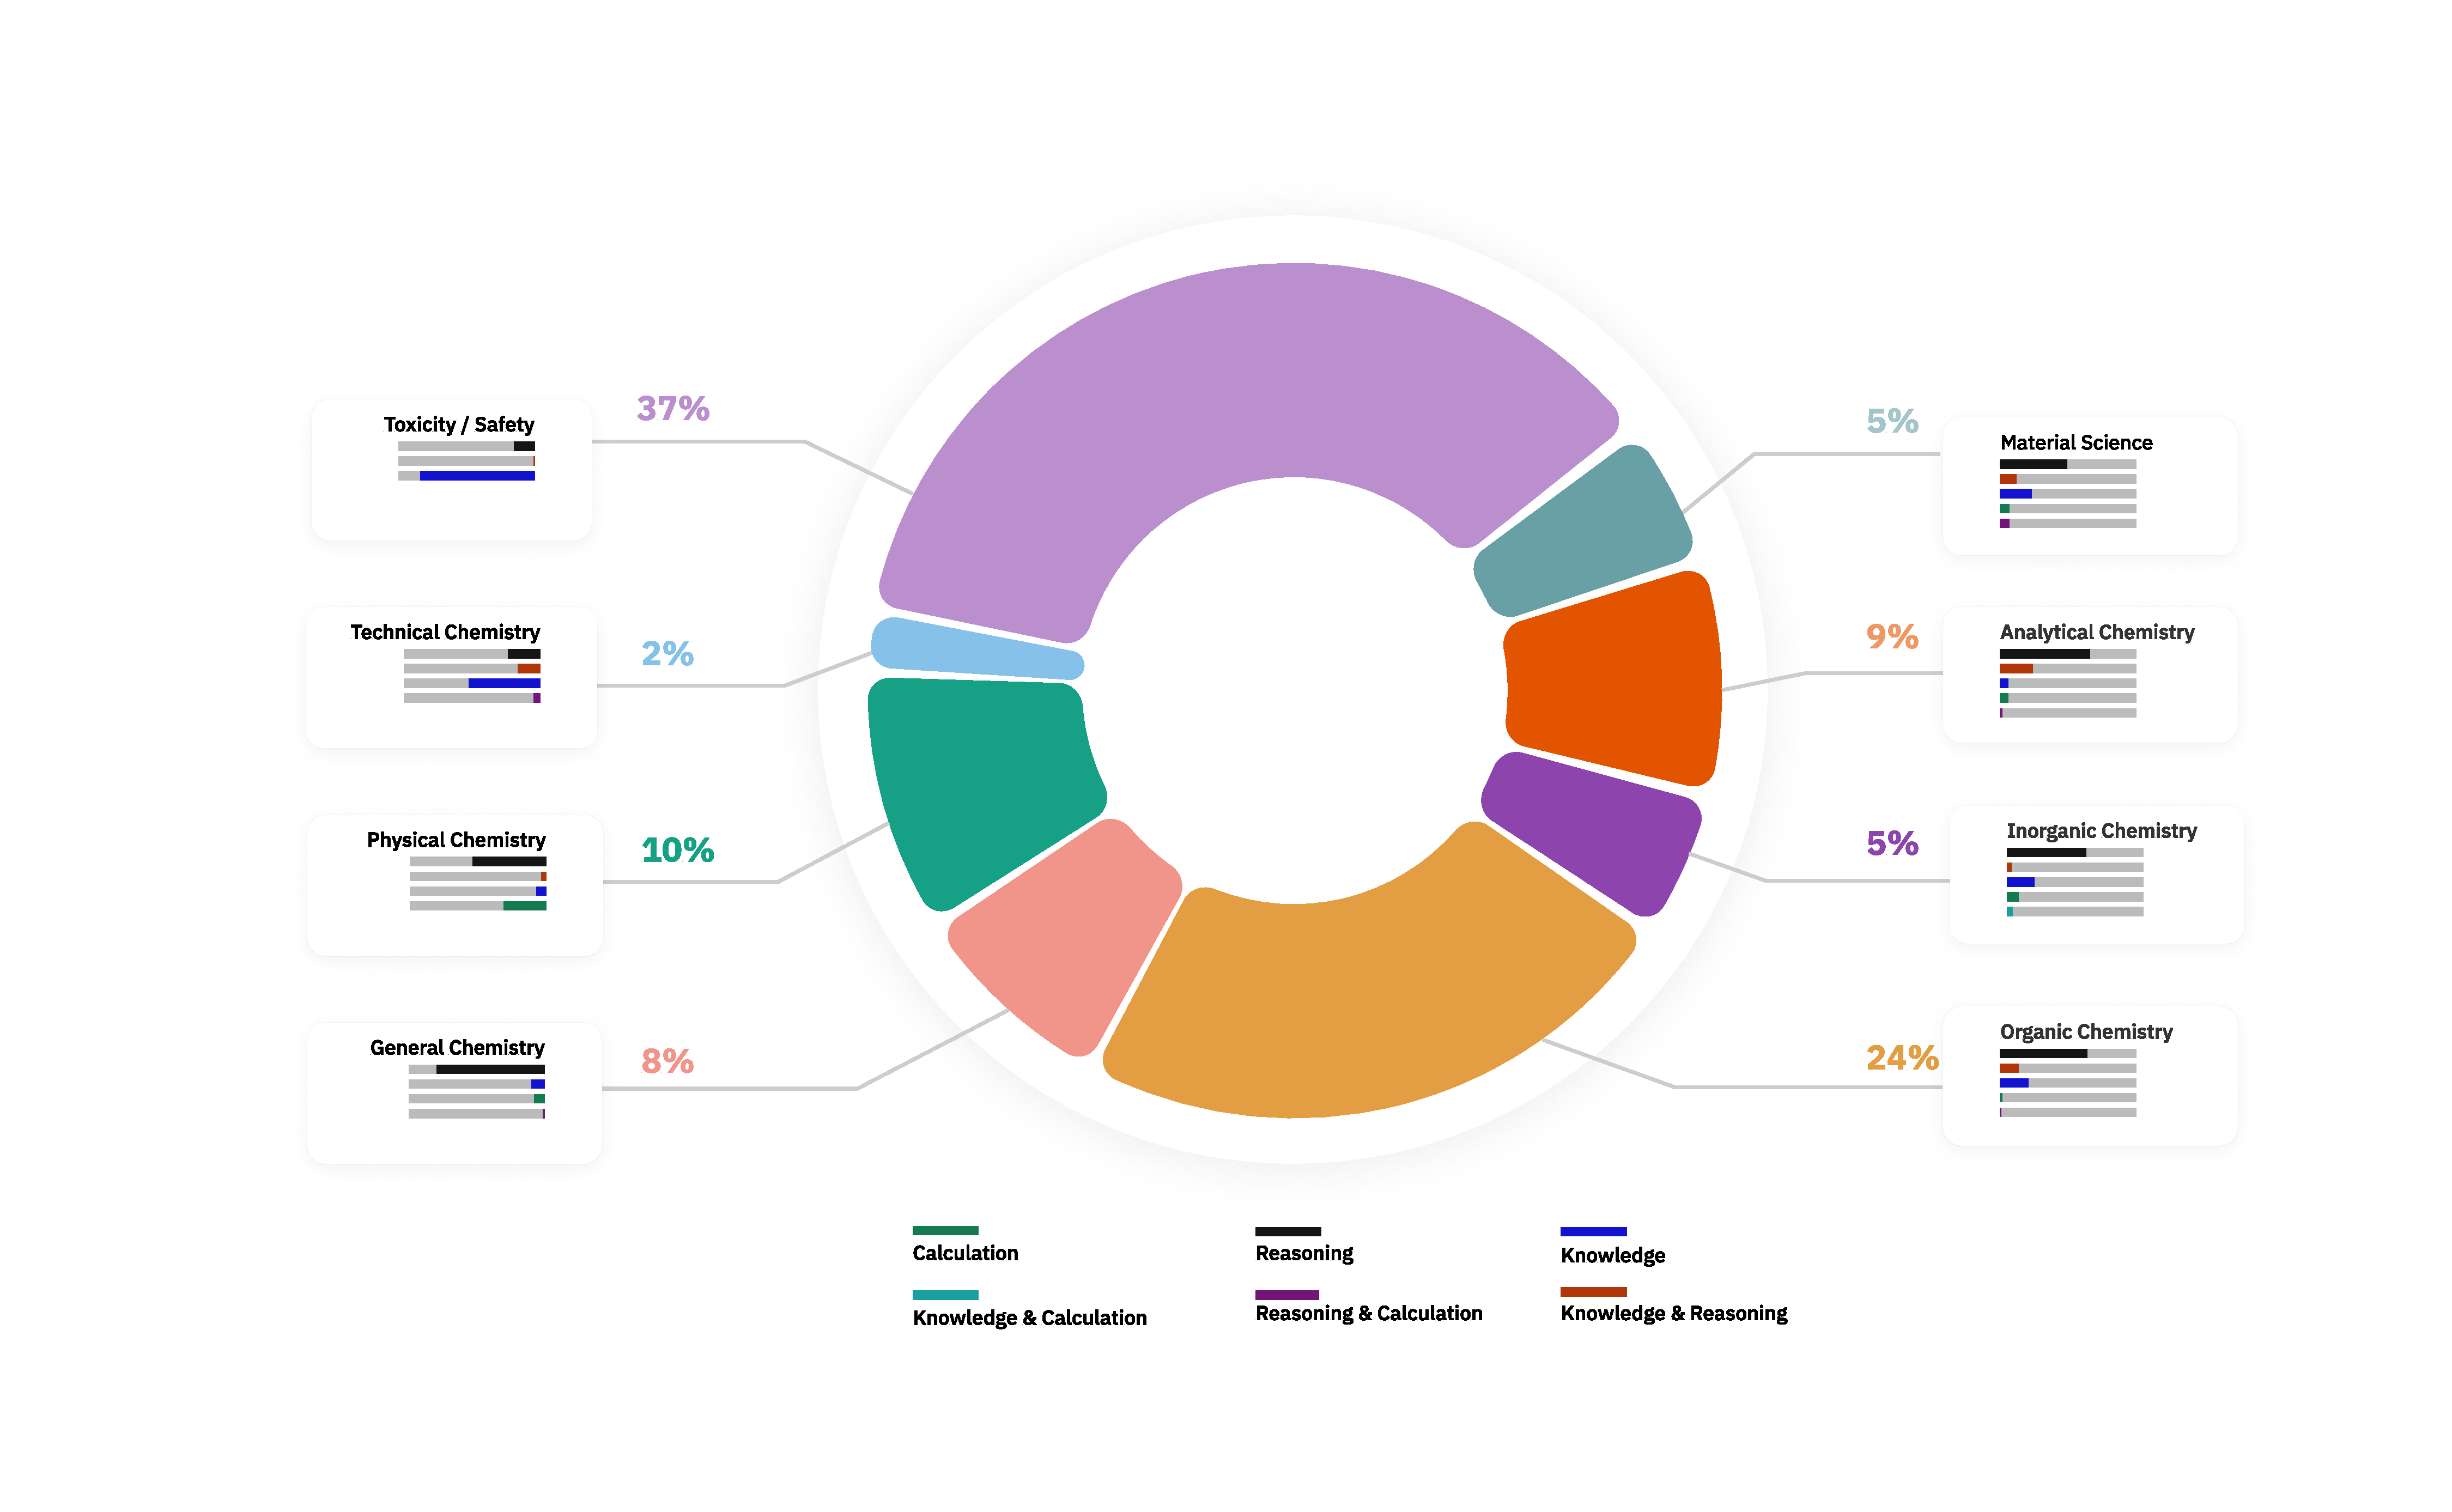
\includegraphics{figures/cb_corpus_v1.pdf}
    \caption{\textbf{Distribution of topics and required skills.} TThis circular plot illustrates the distribution of questions across various chemistry topics, along with the primary skills required to address them. The topics were manually classified, showing a varied representation across different aspects of chemistry. Each topic is associated with a combination of three key skills: Calculation, Reasoning, and Knowledge, as indicated by the colored bars. \chembench samples diverse topics and diverse skills, setting a high bar for \glspl{llm} to demonstrate human-competitive performance across a wide range of chemistry tasks.}
    \label{fig:corpus}
\end{figure}


While many existing benchmarks are designed around \gls{mcq}, this does not reflect the reality of chemistry education and research.
%For this reason, \chembench samples both \gls{mcq} and open-ended questions (\variable{output/mcq_questions.txt} \gls{mcq} questions and \variable{output/non_mcq_questions.txt} open-ended questions).


\paragraph{\enquote{Tiny} subset}
It is important to note that a smaller subset of the corpus might be more practical for routine evaluations.\autocite{polo2024tinybenchmarks}
For instance,~\textcite{liang2023holistic} report costs of more than \$10,000 for \gls{api} calls for a single evaluation on the widely used \gls{helm} benchmark. 
%To address this, we also provide a subset (\variable{output/num_tiny_questions.txt} questions) of the corpus that was curated to be a diverse and representative subset of the full corpus in which topics are more balanced than in the complete corpus (see \Cref{sec:subset-selection} for details on the curation process).
We also used this subset to seed the web application for the human baseline study. 

\begin{figure}
    \centering
    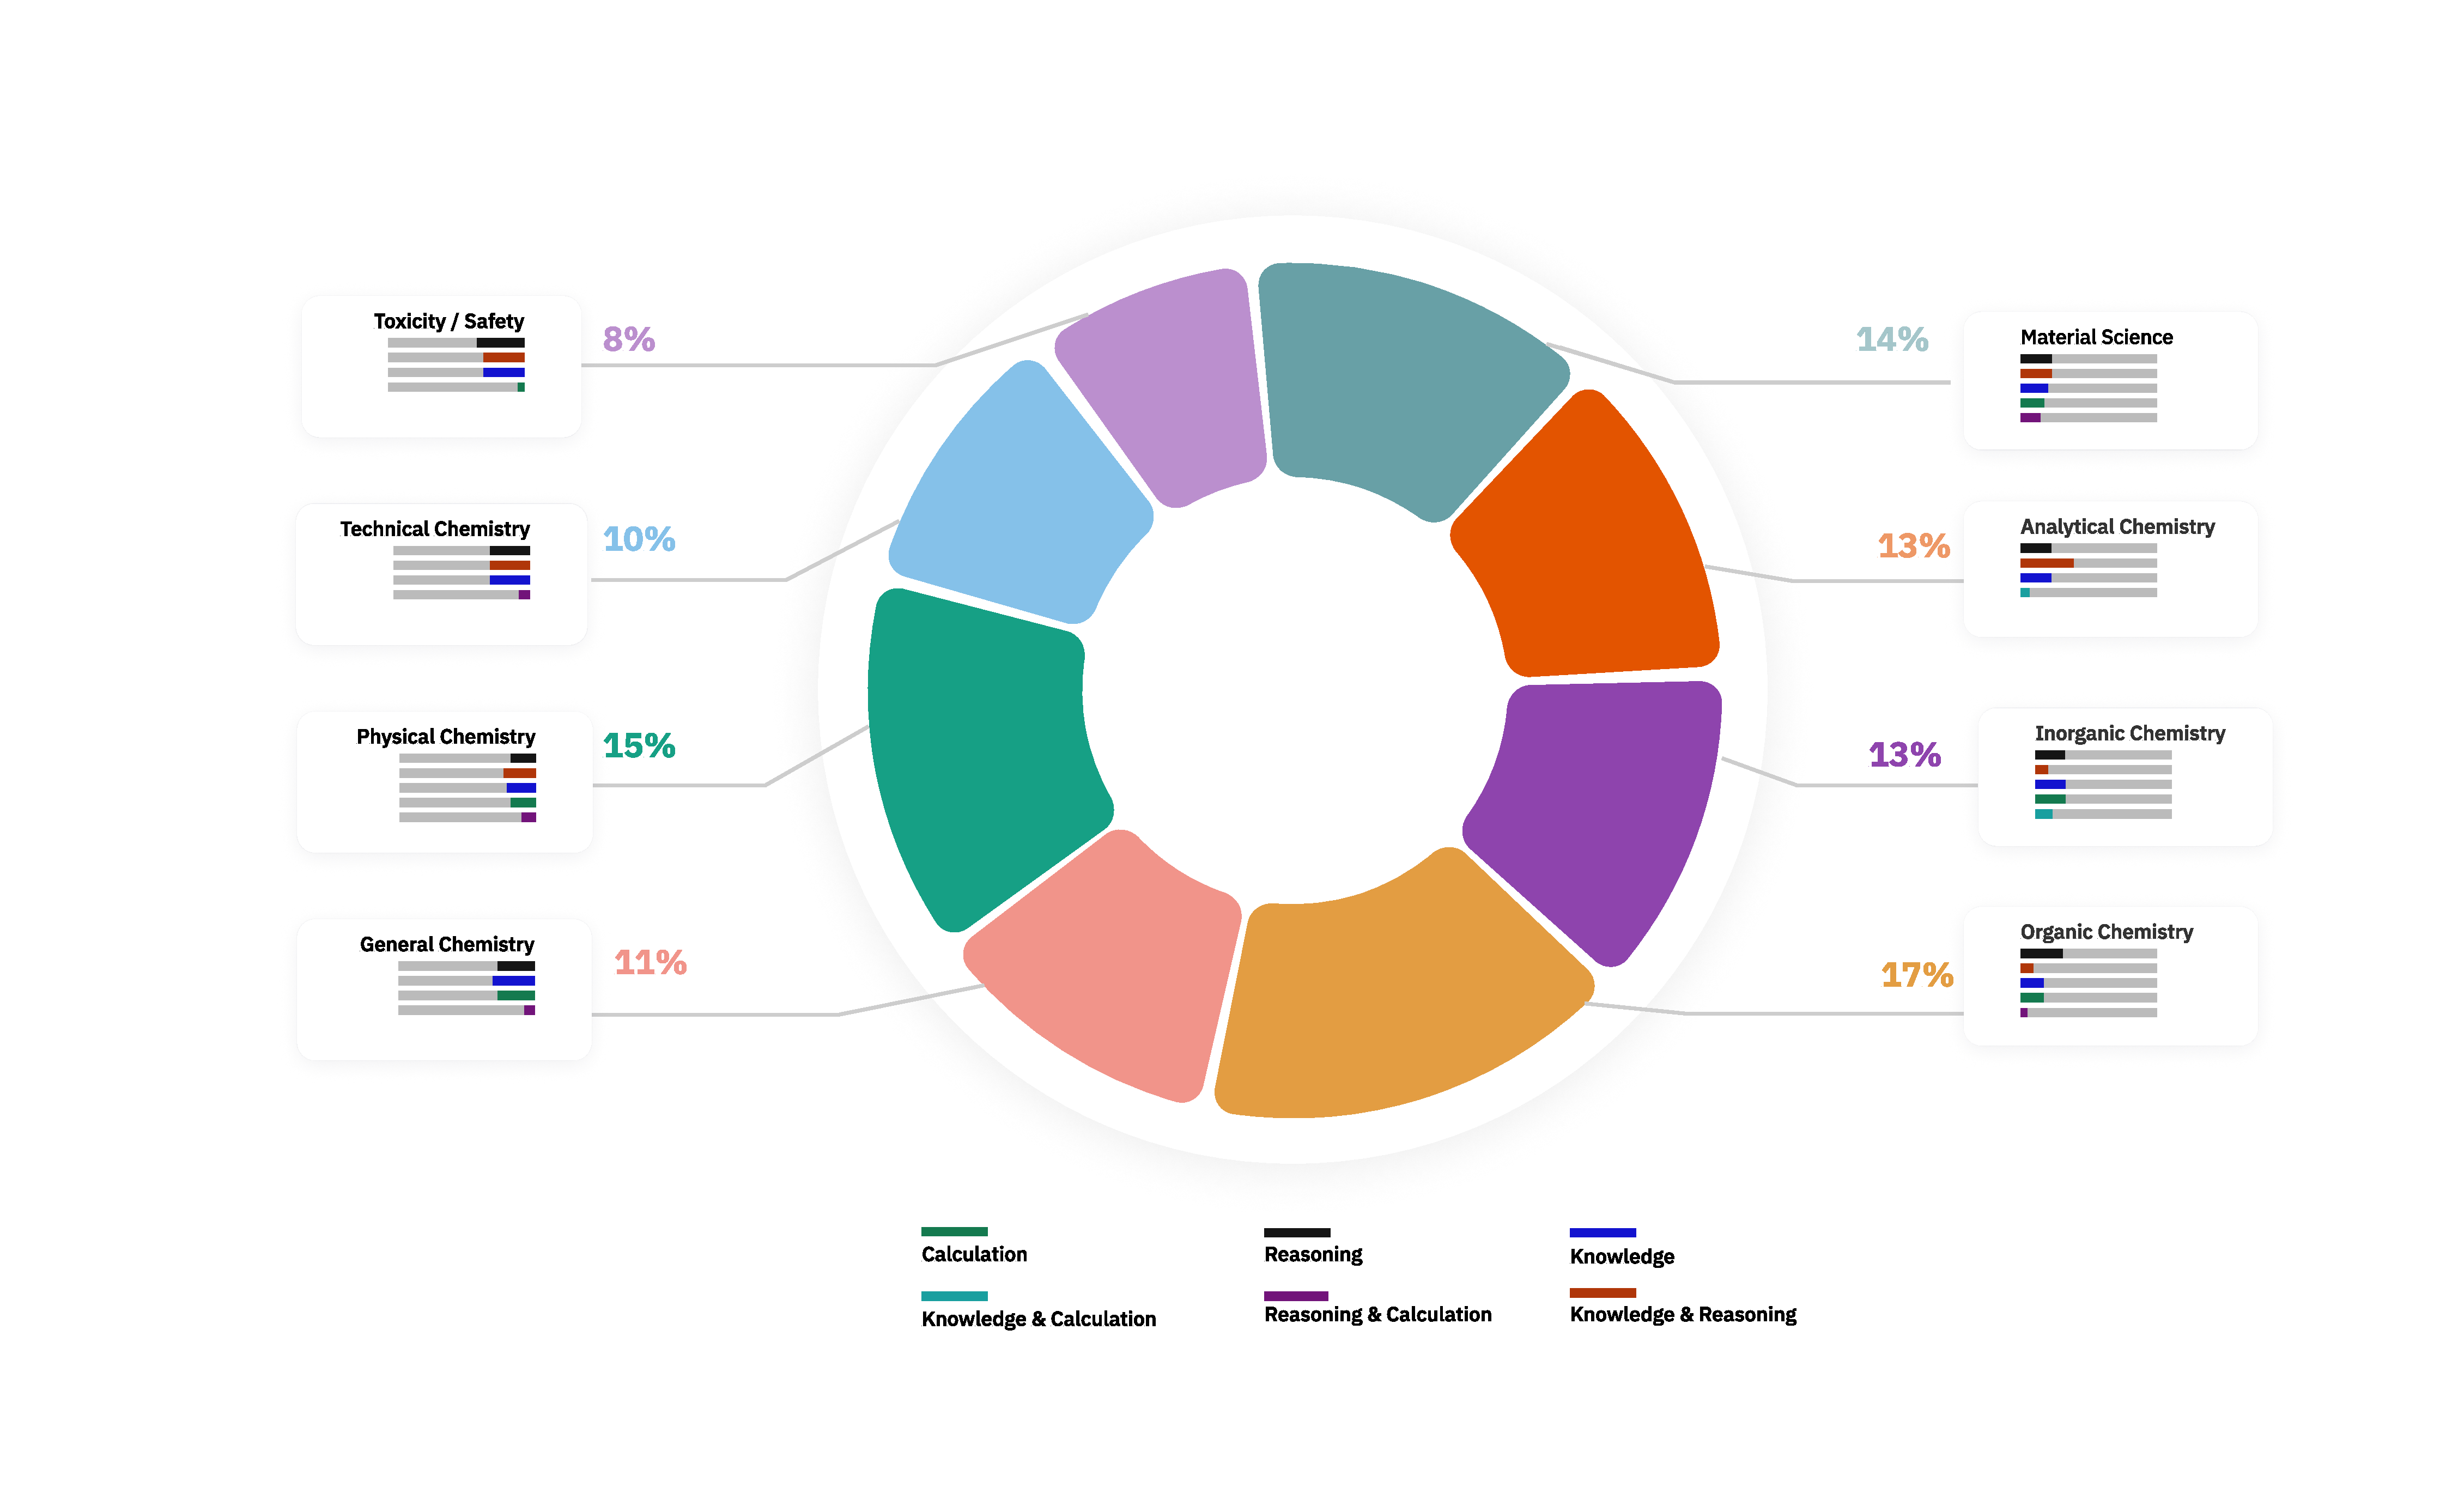
\includegraphics[]{figures/cb_humanset_v1.pdf}
    \caption{\textbf{Composition of the human subset.} The circular plot shows the distribution of topics and required skills in the human subset of the \chembench corpus. The human subset is a representative subset of the full corpus, with a balanced distribution of topics and skills.}
\end{figure}

\subsection{Model evaluation}

\paragraph{Benchmark suite design} Because the text used in scientific settings differs from typical natural language, many models have been developed that deal with such text in a particular way.
For instance, the Galactica model\autocite{taylor2022galactica} uses special tokenization or encoding procedures for molecules and equations. 
Current benchmarking suites, however, do not account for such special treatment of scientific information.
To address this, \chembench encodes the semantic meaning of various parts of the question or answer.  
For instance, molecules represented in \gls{smiles} are enclosed in \texttt{[START\_SMILES][\textbackslash END\_SMILES]} tags. 
This allows the model to treat the \gls{smiles} string differently from other text. 
\chembench can seamlessly handle such special treatment in an easily extensible way because the questions are stored in an annotated format.

Since many widely utilized systems only provide access to text completions (and not the raw model outputs), \chembench is designed to operate on text completions.
This is also important given the growing number of tool-augmented systems that are deemed essential for building chemical copilot systems.
Such systems can augment the capabilities of \glspl{llm} through the use of external tools such as search \glspl{api} or code executors.\autocite{schick2024toolformer, karpas2022mrkl, yao2022react}
In those cases, the \gls{llm} that returns the probabilities for various tokens (that are often used for model evaluations\autocite{Fourrier_Habib_Launay_Wolf}) is only a part of the whole system, and it is not clear how to interpret the probabilities in the context of the whole system.
The text completions, however, are the system's final outputs, which would also be used in a real-world application. 
Hence, we use them for our evaluations.

\begin{figure}[!h]
    \centering
    \includegraphics{figures/human_subset_performance.pdf}
    \caption{\textbf{Performance of models and humans on the \enquote{tiny} subset of the  \chembench corpus.} The figure shows the percentage of questions that the models answered correctly. We use horizontal bars to indicate the performance of various models and highlight statistics of the human performance. 
    Since the humans did not answer all the questions, this plot is based on the subset of questions that most humans answered.
    The evaluation we use here is very strict as it only considers a question answered correctly or incorrectly, partially correct answers are also considered incorrect.
    \Cref{fig:barplot_all_correct_all_questions} provides an overview of the performance of various models on the entire corpus.
    Systems with \enquote{ReAct} in the name are tool augmented, i.e., they can call external tools such as web search or Python code executors to better answer the questions.
    However, we limit those systems to a maximum of ten calls to the \gls{llm}. This constraint led the systems to often not find the correct answer within the specified number of calls.
    In this case, we consider the answer as incorrect. 
    }
    \label{fig:human_vs_models_bar}
    \script{plot_overview_performance_plot.py}
\end{figure}

\paragraph{System performance} 
To understand the current capabilities of \glspl{llm} in the chemical sciences, we evaluated a wide range of leading models\autocite{Huggingface} on the \chembench corpus, including systems augmented with external tools.
An overview of the results of this evaluation is shown in \Cref{fig:human_vs_models_bar}. 
In this figure, we show the percentage of questions that the models answered correctly.
Moreover, we show the worst, best, and average performance of the human experts in our study, which we obtained via a custom web application (\url{chembench.org}) that we used to survey the experts.
Remarkably, the figure shows that the leading \gls{llm}, Claude 3, outperforms the best human in our study in this overall metric and vastly, by more than a factor of two, exceeds the average performance of the experts in our study.
Many other models also outperform the average human performance. 
Interestingly, the Galactica model, which was trained specifically for scientific applications, underperformed compared to many advanced commercial and some open-source models and barely exceeds the random baseline.

Given the considerable interest in tool-augmented systems, the mediocre performance of these systems (GPT-3.5 and Claude 2 augmented with tools) in our benchmark is striking. 
Their lack of performance, however, is partially because we limited the system to a maximum of ten \gls{llm} calls.
With the default tool augmented setup (using the so-called ReAct method\autocite{yao2022react}), however, this often did not allow the system to identify the correct answer (e.g., because it repeatedly tried to search for the answer on the web and did not find a solution within ten calls to the \gls{llm}).
This observation highlights the importance of communicating and measuring not only predictive performance but also computational cost (e.g., in terms of \gls{api} calls) for tool-augmented systems.


\paragraph{Performance per topic} To obtain a more detailed understanding of the performance of the models, we also analyzed the performance of the models in different subfields of the chemical sciences.
For this analysis, we defined a set of topics (see \Cref{sec:meth-topic}). We classified all questions in the \chembench corpus into these topics based on hand-crafted rules and classifier models operating on the question texts.
We then computed the percentage of questions the models or humans answered correctly for each topic.
\begin{figure}[!h]
    \centering
    \includegraphics{figures/all_questions_models_completely_correct_radar_human.pdf}
    \caption{\textbf{Performance of the models and humans on the different topics of the \enquote{tiny} subset of the \chembench corpus.} The radar plot shows the performance of the models and humans on the different topics of \enquote{tiny} subset of the \chembench corpus. The performance is measured as the fraction of questions that were answered completely correctly by the models.
    The best score for every dimension is one (all questions answered correctly), and the worst is zero (no question answered correctly). A larger colored area indicates a better performance.
    This figure shows the performance on the subset of questions that were answered by humans. The performance of models on the entire corpus is shown in \Cref{fig:performance_per_topic}.
    }
    \label{fig:all_questions_models_completely_correct_radar_human}
    \script{analyze_model_reports.py}
\end{figure}


% In this spider chart, the worst score for every dimension is zero (no question answered correctly), and the best score is one (all questions answered correctly). 
% Thus, a larger colored area indicates a better performance. 
% One can observe that this performance varies widely across models and topics. 
% While macromolecular chemistry and biochemistry receive relatively high scores for many models, this is not the case for topics such as chemical safety or analytical chemistry.
% In the subfield of analytical chemistry the prediction of the number of signals observable in a \gls{nmr} spectrum proved difficult for the models (e.g., \variable{output/subset_scores/is_number_nmr_peaks_gpt4.txt} percent correct answers for GPT-4) while this question appeared easier (\variable{output/human_subset_scores/is_number_nmr_peaks.txt} percent correct) for trained humans.
% Importantly, the human experts are given a drawing of the compounds, whereas models are only shown the \gls{smiles} string of a compound and have to use this to reason about the symmetry of the compound (i.e., to identify the number of diasterotopically distinct protons, which requires \emph{reasoning} about the topology and structure of a molecule). 
% These findings also shine an interesting light on the value of textbook-inspired questions. 
% A subset of the questions in the \chembench are based on textbooks targeted at undergraduate students. 
% On those questions, the models tend to perform better than on some of our semi-automatically constructed tasks (see \Cref{fig:performance_per_topic}).
% For instance, while the overall performance in the chemical safety topic is low, the models would pass the certification exam according to the German Chemical Prohibition Ordinance based on a subset of questions we sampled from the corresponding question bank (e.g., \variable{output/subset_scores/is_gfk_gpt4.txt}\% correct answers for GPT-4, \variable{output/subset_scores/is_gfk_claude3.txt}\% for Claude 3, and \variable{output/human_subset_scores/is_gfk.txt}\% for the human experts).
% While those findings are impacted by the subset of questions we sampled, the results still highlight that good performance on such question bank or textbook questions does not necessarily translate to good performance on other questions that require more reasoning.

% We also gain insight into the models' struggles with chemical reasoning tasks when we examine their performance as a function of molecular descriptors.
% If the model would answer questions after reasoning about the structures, one would expect the performance to depend on the complexity of the molecules.
% However, we find that the models' performance does not correlate with complexity indicators but rather trivially with the size of the compounds (see \Cref{tab:correlation_coefficients}).
% This indicates that the models may not be able to reason about the structures of the molecules (in the way one might expect) but instead rely on retrieval of fragments of the training data.
% Those observations mirror recent findings that \glspl{llm} struggle to \enquote{reverse} facts they have seen in training (i.e., generalize from \enquote{A has feature B} to \enquote{B is a feature of A}).\autocite{berglund2023reversal, zhu2023physics, allen2023physics, golovneva2024reverse}

% It is important to note that the model performance for some topics, however, is underestimated in the current evaluation. 
% This is because models provided via \glspl{api} typically have safety mechanisms that prevent them from providing answers that the provider deems unsafe.
% For instance, models might refuse to provide answers about cyanides. 
% To overcome this, direct access to the model weights would be required, and we strive to collaborate with the developers of frontier models to overcome this limitation in the future.
% This is facilitated with the tooling \chembench provides, thanks to which contributors can automatically add new models in an open science fashion.

\paragraph{Judging chemical preference}

One interesting finding of recent research is that foundation models can judge interestingness.\autocite{zhang2024omniopenendednessmodelshuman}
If models could do so for chemical compounds, this would open opportunities for novel optimization approaches. 
Such open-ended tasks, however, depend on an external observer defining what interestingness is.\autocite{hughes2024openendednessessentialartificialsuperhuman}
Here, we posed models the same question~\textcite{Choung_2023} asked chemists at a drug company: \enquote{Which of the two compounds do you prefer?} (in the context of an early virtual screening campaign setting).
While chemists showed a fair degree of interrater agreement, most of our models do not correlate with the preferences of expert chemists---even if they perform well on many other tasks in \chembench.
This indicates that using preference tuning for chemical settings is a promising approach to explore in future research.


% Estimate of difficulty
\paragraph{Confidence estimates} One might wonder whether the models can estimate if they can answer a question correctly. 
If they could do so, incorrect answers would be less problematic as one could detect when an answer is incorrect.

REWRITE 

%To investigate this, we prompted\autocite{xiong2023llms} some of the top-performing models to estimate, on an ordinal scale, their confidence in their ability to answer the question correctly.

% \begin{figure}[!h]
%     \centering
%     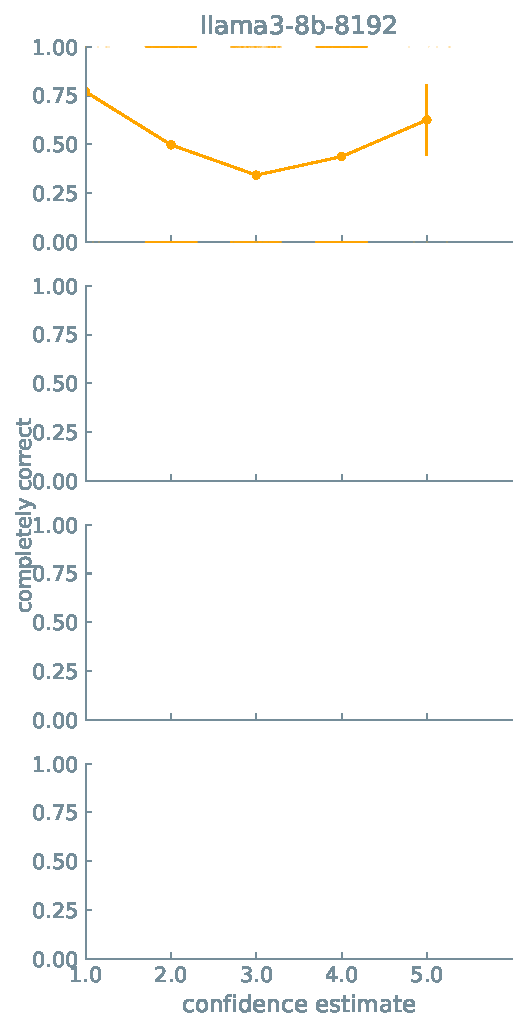
\includegraphics{figures/confidence_vs_performance_overall.pdf}
%     \caption{\textbf{Relationship between confidence of the model in the answer and correctness.} For this analysis, we used verbalized confidence estimates from the model. We prompted the models to return a confidence score on an ordinal scale to obtain those estimates. We then plot the correctness of the answers (which is calculated as the mean value of all answers being either correct (1) or incorrect (0)) against the confidence score.
%         The stripplots show the individual data points, a strong density indicating a higher number of points. The lines show the mean, and the error bars show the standard error of the mean. The figure shows that the reliability of the confidence estimates varies widely across models. While the ones for GPT-4 and Claude 2 are not particularly reliable, the ones for Claude 3 follow the expected trend better.}
%     \label{fig:confidence_vs_performance}
%     \script{joint_analysis_confidence_performance.py}
% \end{figure}

% In \Cref{fig:confidence_vs_performance}, we show that for some models, there is no significant correlation between the estimated difficulty and whether the models answered the question correctly or not.
% For applications in which humans might rely on the models to provide answers, this is a concerning observation highlighting the need for critical reasoning in the interpretation of the model's outputs.\autocite{Li_2023, miret2024llms}
% For example, for the questions about the safety profile of compounds, GPT-4 reported an average confidence of \variable{output/model_confidence_performance/gpt4_is_pictograms_average_confidence_correct_overall.txt} (on a scale of 1--5) for the \variable{output/model_confidence_performance/gpt4_is_pictograms_num_correct_overall.txt} questions it answered correctly and \variable{output/model_confidence_performance/gpt4_is_pictograms_average_confidence_incorrect_overall.txt} for the \variable{output/model_confidence_performance/gpt4_is_pictograms_num_incorrect_overall.txt} questions it answered incorrectly.
% While, on average, the verbalized confidence estimates from Claude 3 seem better calibrated (\Cref{fig:confidence_vs_performance}), they are still misleading in some cases. 
% For example, for the questions about \gls{ghs} pictograms Claude 3 returns an average score of \variable{output/model_confidence_performance/claude3_is_pictograms_average_confidence_correct_overall.txt} for correct answers and \variable{output/model_confidence_performance/claude3_is_pictograms_average_confidence_incorrect_overall.txt} for incorrect answers.

\section{Conclusions}
On the one hand, our findings underline the impressive capabilities of \glspl{llm} in the chemical sciences: Leading models outperform domain experts in specific chemistry questions on many topics. 
On the other hand, there are still striking limitations. 
For very relevant topics the answers models provide are wrong. 
On top of that, many models are not able to reliably estimate their own limitations.
Yet, the success of the models in our evaluations perhaps also reveals more about the limitations of the exams we use to evaluate models---and chemists---than about the models themselves.
For instance, while models perform well on many textbook questions, they struggle with questions that require some more reasoning. 
Given that the models outperformed the average human in our study, we need to rethink how we teach and examine chemistry.
Critical reasoning is increasingly essential, and rote solving of problems or memorization of facts is a domain in which \glspl{llm} will continue to outperform humans.

Our findings also highlight the nuanced trade-off between breadth and depth of evaluation frameworks. 
The analysis of model performance on different topics shows that models' performance varies widely across the subfields they are tested on. 
However, even within a topic, the performance of models can vary widely depending on the type of question and the reasoning required to answer it.

The current evaluation frameworks for chemical \glspl{llm} are primarily designed to measure the performance of the models on specific property prediction tasks. 
They cannot be used to evaluate reasoning or systems built for scientific applications. 
Thus, we had little understanding of the capabilities of \glspl{llm} in the chemical sciences.
Our work shows that carefully curated benchmarks can provide a more nuanced understanding of the capabilities of \glspl{llm} in the chemical sciences.
Importantly, our findings also illustrate that more focus is required in developing better human-model interaction frameworks, given that models cannot estimate their limitations.

While our findings indicate many areas for further improvement of \gls{llm}-based systems, it is also important to realize that clearly defined metrics have been the key to the progress of many fields of \gls{ml}, such as computer vision. 
Although current systems are far from reasoning like a chemist, our \chembench framework will be a stepping stone for developing systems that might come closer to this goal.

\clearpage

\section{Methods}

\subsection{Curation workflow}\label{sec:curation}
For our dataset, we curated questions from existing exams or exercise sheets but also programmatically created new questions.
Questions were added via Pull Requests on our GitHub repository and only merged into the corpus after passing manual review (\Cref{fig:curation_workflow}) as well as automated checks (e.g., for compliance with a standardized schema).

To ensure that the questions do not enter a training dataset, we use the same canary string as the BigBench project.
This requires that \Gls{llm} developers filter their training dataset for this canary string.\autocite{openai2024gpt4, srivastava2022beyond}

\begin{figure}[!h]
    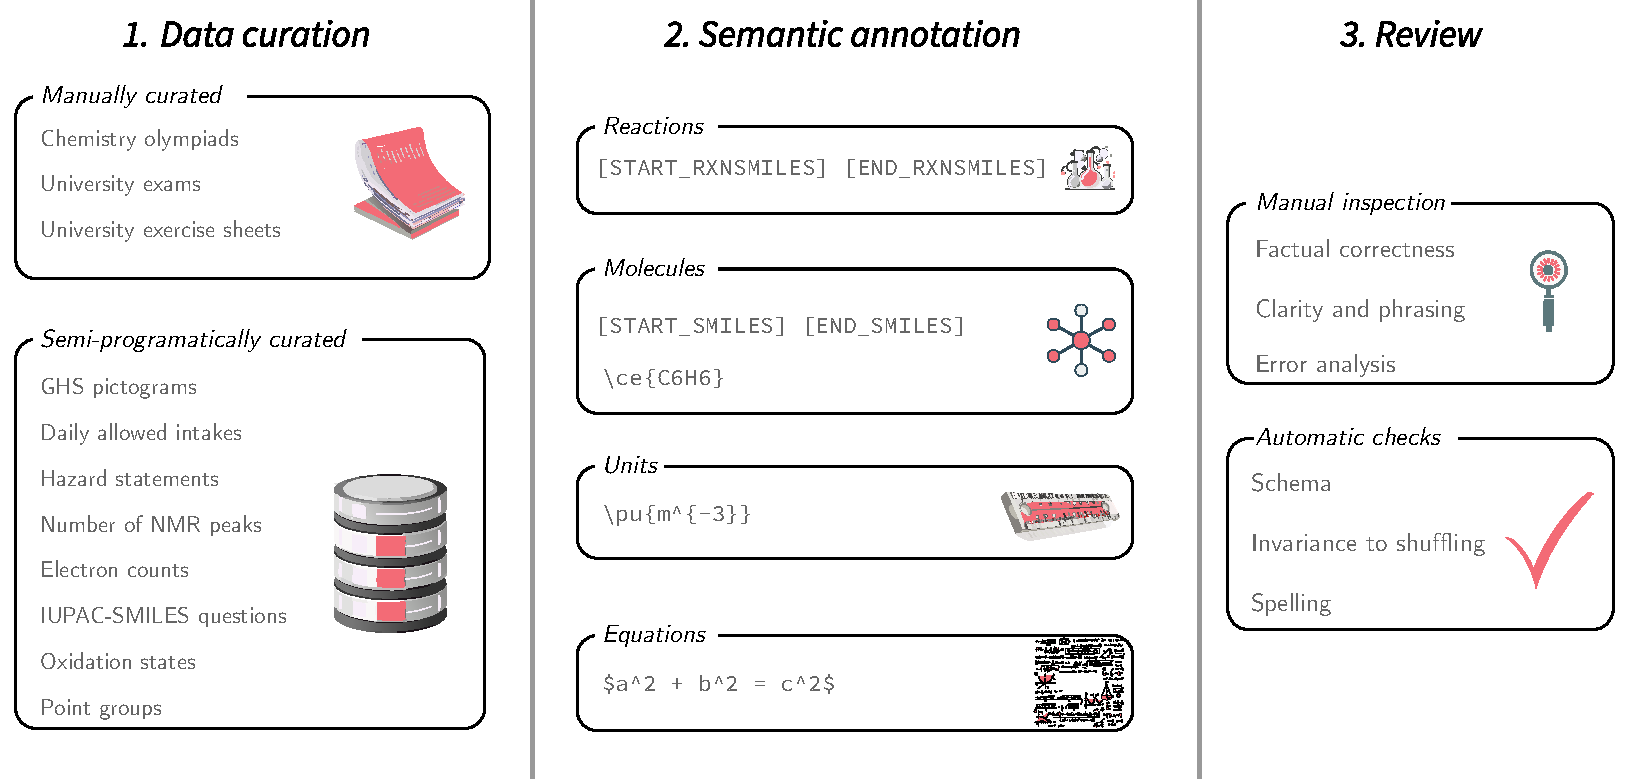
\includegraphics[width = \textwidth]{figures/chem-bench.pdf}
    \caption{\textbf{Overview of the workflow for the assembly of the \chembench corpus}. 
    To assemble the \chembench corpus, we first collected questions from various sources. Some tasks were manually curated, others semi-programmatically. We added semantic annotations for all questions to make them compatible with systems that use special processing for modalities that are not conventional natural text. We reviewed the questions using manual and automatic methods before adding them to the corpus.}
    \label{fig:curation_workflow}
\end{figure}

\paragraph{Manually curated questions}
Manually curated questions were sourced from various sources, including university exams, exercises, and question banks. \Cref{tab:manually_sources} provides an overview of the sources of the manually curated questions.

%\begin{table}[h]
    \begin{tabularx}{\textwidth}{p{3.5 cm}p{6.5 cm}p{.5cm}X}
    \toprule
    source & description & question count \\
    \midrule
NMR spectroscopy & Questions are based on images shared via the Twitter account \href{https://twitter.com/NMRspectroscopy}{NMRspectroscopy} && 5 \\
\midrule
Analytical chemistry & Questions are based on exercises in master student examination at the FSU Jena, Germany &&  \variable{output/question_count_per_dir/json_file_counts_analytical_chemistry.txt} \\
\midrule
\multirow{2}{*}{General chemistry} & Questions originate from examinations for grade 10 at the Marist Comprenhensive Academy Uturu, Nigeria && \variable{output/question_count_per_dir/json_file_counts_Gen_Chem_MCA.txt} \\
 & Questions originate from the Bachelor of Science (for chemistry) courses at the TUM, Germany && \variable{output/question_count_per_dir/json_file_counts_ac_faessler_tum.txt} + \variable{output/question_count_per_dir/json_file_counts_pum_tum.txt} \\
 \midrule
Functional materials and  nanomaterials & Questions are based on exercises in a seminar conducted at the FSU Jena, Germany && \variable{output/question_count_per_dir/json_file_counts_func_mats_and_nanomats.txt} \\
\midrule
Combustion engineering & Based on a Master of Science examination paper at the University of Magdeburg, Germany && \variable{output/question_count_per_dir/json_file_counts_combustion_engineering.txt} \\
\midrule
Materials' synthesis & Questions are based on seminars on material synthesis from FSU Jena, Germany && \variable{output/question_count_per_dir/json_file_counts_materials_synthesis.txt} \\
\midrule
Chemistry olympiad & National and International Olympiads held in US, UK and Moldova && \variable{output/question_count_per_dir/json_file_counts_icho.txt} \\
\midrule
Organic reactivity & Based on exams in the Bachelor of Science in Chemistry at the TUM, Germany && \variable{output/question_count_per_dir/json_file_counts_organic_reactivity.txt} \\
\midrule
Periodic table & Manually created && \variable{output/question_count_per_dir/json_file_counts_periodic_table_properties.txt} \\
\midrule
Polymer chemistry & Based on examinations at the University of Hamburg, Germany && \variable{output/question_count_per_dir/json_file_counts_polymer_chemistry.txt} \\
\midrule
Textbook questions & Various textbooks covering biomolecular science, drug synthesis, molecular structure, organic chemistry, and X-ray crystallography && \variable{output/question_count_per_dir/json_file_counts_oup.txt} \\
\midrule
Safety & Based on the question bank published by the Federal/State Working Group  on Chemical Safety (BLAC), which is used for the expertise examination (“Sachkundepr\"ufung”) && \variable{output/question_count_per_dir/json_file_counts_blac_gfk.txt} \\
       & Based on toxicology exams at the LMU Munich, Germany && \variable{output/question_count_per_dir/json_file_counts_LMU_tox.txt} \\
       & Based on toxicology exams at the University of Vienna, Austria && \variable{output/question_count_per_dir/json_file_counts_tox_pharma_vienna.txt} \\
       & Based on toxicology exams at WWU Munster, Germany && \variable{output/question_count_per_dir/json_file_counts_tox_wwu.txt} \\
       & Based on exercises for lectures in high-energy density materials at LMU Munich, Germany && \variable{output/question_count_per_dir/json_file_counts_hedm_munich.txt} \\
       & Based on pharmacology exams at the University of Vienna, Austria && \variable{output/question_count_per_dir/json_file_counts_pharmacology_vienna.txt} \\
\bottomrule
\end{tabularx}
\end{table}




\paragraph{Semi-programmatically generated questions}
In addition to the manually curated questions, we also generated questions programmatically. An overview of the sources of the semi-programmatically generated questions is provided in \Cref{tab:semi_programatically_sources}.


%\begin{table}[h]
\begin{tabularx}{\textwidth}{Xp{7 cm}X}
    \toprule
    source & description & question count \\
\midrule
Number of isomers & MAYGEN was used to compute the number of isomers for a set of SMILES extracted from the ZINC dataset. & \variable{output/question_count_per_dir/json_file_counts_number_of_isomers.txt} \\
Total electron count of molecules & Electron counts based on the data from https://www.cheminfo.org/. & \variable{output/question_count_per_dir/json_file_counts_electron_counts.txt} \\
Oxidation states & Oxidation states questions based on the data from https://www.cheminfo.org/. & \variable{output/question_count_per_dir/json_file_counts_oxidation_states.txt} \\
Chemical reactivity & Questions are framed based on the information from Cameo Chemicals website (https://cameochemicals.noaa.gov/reactivity). & \variable{output/question_count_per_dir/json_file_counts_reactive_groups.txt} \\
Number of NMR signals & Molecules are sampled from the ZINC database and the number of NMR signals is computed with OpenChemLib & \variable{output/question_count_per_dir/json_file_counts_number_of_nmr_peaks.txt} \\
Point group of molecules & Our ChemCaption tool is used to assign the point group, and then each case was manually checked to select well defined cases. & \variable{output/question_count_per_dir/json_file_counts_point_group.txt} \\
IUPAC-SMILES pairs & Sampled from the PubChem database & \variable{output/question_count_per_dir/json_file_counts_smiles_to_name.txt} + \variable{output/question_count_per_dir/json_file_counts_smiles_to_name.txt} \\
\multirow{3}{*}{PubChem safety data} & Daily allowable intakes according to the World Health Organization & \variable{output/question_count_per_dir/json_file_counts_dai.txt}  \\
 & Definitions of hazard statements &  \variable{output/question_count_per_dir/json_file_counts_h_statements.txt} \\
 & GHS classification of chemicals mined through the API & \variable{output/question_count_per_dir/json_file_counts_pictograms.txt} \\
\multirow{2}{*}{Safety}
& Materials' compatibility & \variable{output/question_count_per_dir/json_file_counts_materials_compatibility.txt} \\
 & Chemical compatibility & \variable{output/question_count_per_dir/json_file_counts_chem_chem_comp.txt} \\
\bottomrule
\end{tabularx}
\end{table}



\clearpage

\subsection{Model evaluation workflow}
EXPAND THIS section. 

\paragraph{Prompting}

We employ distinct prompt templates tailored for completion and instruction-tuned models to maintain consistency with the training. 
As explained below, we impose constraints on the models within these templates to receive responses in a specific format so that robust, fair, and consistent parsing can be performed.
Certain models are trained with special annotations and \LaTeX\xspace syntax for scientific notations, chemical reactions, or symbols embedded within the text. 
For example, all the SMILES representations are encapsulated within \texttt{[START\_SMILES][\textbackslash END\_SMILES]} in Galactica\autocite{taylor2022galactica}.
Our prompting strategy consistently adheres to these details in a model-specific manner by post-processing \LaTeX\xspace syntax, chemical symbols, chemical equations, and physical units (by either adding or removing wrappers).
This step can be easily customized in our codebase.



\paragraph{Parsing}
Our parsing workflow is multistep and primarily based on regular expressions.
In the case of instruction-tuned models, we first identify the \texttt{[ANSWER]}\texttt{[\textbackslash ANSWER]} environment we prompt the model to report the answer in.
In the case of completion models, this step is skipped. From there, we attempt to extract the relevant enumeration letters (for multiple-choice questions) or numbers.
In the case of numbers, our regular expression was engineered to deal with various forms of scientific notation.
As initial tests indicated that models sometimes return integers in the form of words, e.g., \enquote{one} instead of \enquote{1}, we also implemented a word-to-number conversion using regular expressions.
If these hard-coded parsing steps fail, we use a \gls{llm}, e.g., Claude 2, to parse the completion.


\paragraph{Models}
Rewrite - as table. The table can then also contain if it has been completion or instruction-prompted.

\subsection{Confidence estimate}
To estimate the models' confidence, we prompted them with the question (and answer options for \gls{mcq}) and the task to rate their confidence to produce the correct answer on a scale from 1 to 5. 
We decided to use verbalized confidence estimates\autocite{xiong2023llms} since we found those closer to current practical use cases than other prompting strategies, which might be more suitable when implemented in systems.

\subsection{Human baseline}


\paragraph{Question selection} \label{sec:subset-selection}
Rewrite.

\paragraph{Study design}
Rewrite.

\paragraph{Participants}
% Users were open to reporting about their experience in chemistry. 
% Overall, \variable{output/num_users_with_education_info.txt} did so. 
% Out of those, \variable{output/num_human_phd.txt} reported to have been awarded a Ph.D.
% \variable{output/num_human_postdoc.txt} are beyond a first postdoc, \variable{output/num_human_master.txt} have a master's degree, and \variable{output/num_human_bachelor.txt} have a bachelor's degree.


\paragraph{Comparison with models}
%To compare the performance of humans (who might have answered only some questions) with the performance of models (which answered all questions), we focussed on questions that at least four humans answered and limited the pool of human scorers to those who answered at least 100 questions (i.e., \variable{output/num_humans_with_more_than_100_scores.txt} humans). 
%The latter threshold was chosen to limit it to humans who seriously attempted to answer a part of the questions systematically. 
%This analysis might lead to potential biases, most likely in favor of humans, as they were allowed to skip questions. \variable{output/num_humans_with_204_scores.txt} humans answered more than 200 questions.
For the analysis, we treated each human as a model. We computed the topic aggregated averages per human for analyses grouped by topic and then averaged over all humans.

\subsection{Classification of questions into topics}\label{sec:meth-topic} 
% When curating our dataset, we systematically recorded keywords and sources.
% To allow for analysis of the model performance as a function of the topic, we leverage this information together with the output of sequence classification models.
% We use this information to make the assignment for questions that can easily be assigned to a topic based on the source (e.g., number of \gls{nmr} signals, chemical compatibility, toxicology exam questions).
% For the remaining ones, e.g., from chemistry olympiad questions, we use zero-short sequence classification\autocite{zeroshotsequence} using the BART model\autocite{bart, FacebookBART}, which our preliminary analysis found to be more robust than topic modeling based on embeddings from OpenAI's \texttt{ada} model or Cohere's \texttt{Cohembed-english-v3.0} model.

REWRITE. 

\section*{Data and code availability}
The code and data for \chembench is available at \url{https://github.com/lamalab-org/chem-bench}.
The code for the app for our human baseline study is available at \url{https://github.com/lamalab-org/chem-bench-app}. 
To ensure reproducibility, this manuscript was generated using the \href{https://show-your.work/en/latest/}{\showyourwork} framework.\autocite{Luger2021}
The code to rebuild the paper (including code for all figures and numbers next to which there is a GitHub icon) can be found at \url{\GitHubURL}. 
To facilitate reproduction, some intermediate analysis results are cached at \url{http://dx.doi.org/10.5072/zenodo.34706}.

\section*{Acknowledgements}
This work was supported by the Carl Zeiss Foundation, a \enquote{Talent Fund} of the \enquote{Life} profile line of the Friedrich Schiller University Jena.
We also thank Stability.AI for the access to its HPC cluster and donations. In addition, M.S-W.'s work was supported by Intel and Merck via the AWASES programme. 
K.M.J.\ is part of the NFDI consortium FAIRmat funded by the Deutsche Forschungsgemeinschaft (DFG, German Research Foundation) – project 460197019.

M.A.\ expresses gratitude to the European Research Council (ERC) for evaluating the project with the reference number 101106377 titled \enquote{CLARIFIER} and accepting it for funding under the HORIZON TMA MSCA Postdoctoral Fellowships - European Fellowships. 
Furthermore, M.A.\ acknowledges the funding provided by UK Research and Innovation (UKRI) under the UK government’s Horizon Europe funding guarantee (Grant Reference: EP/Y023447/1; Organization Reference: 101106377).

M.R.\ and U.S.S.\ thanks the \enquote{Deutsche Forschungsgemeinschaft} for funding under the regime of the priority programme SPP 2363 \enquote{Utilization and Development of Machine Learning for Molecular Applications – Molecular Machine Learning} (SCHU 1229/63-1; project number 497115849).

In addition, we thank the OpenBioML.org community and their ChemNLP project team for valuable discussions.
Moreover, we thank Pepe Márquez for discussions and support and Julian Kimmig for feedback on the web app. 
In addition, we acknowledge support from Sandeep Kumar with an initial prototype of the web app.
We thank Bastian Rieck for developing the \LaTeX-credit package (\url{https://github.com/Pseudomanifold/latex-credits}) and thank Berend Smit for feedback on an early version of the manuscript.

\section*{Conflicts of interest}
K.M.J.\ was a paid consultant for OpenAI (as part of the red teaming network). M.P.\ is an employee of Stability.AI, and A.M.\ and N.A.\ were paid contractors of Stability.AI.

\section*{Author contributions}

\scriptsize
\insertcredits
\normalsize
\printbibliography
\end{refsection}

\clearpage
\begin{refsection}
\appendix
\section{Appendix}

\subsection{Desired properties of a chemistry benchmark} \label{sec:desired-properties}

\begin{itemize}
    \item \emph{End-to-end automation}. For model development, the evaluations must be run many times (e.g., on regular intervals of a training run).
    Approaches that rely on humans scoring the answers of a system\autocite{Schulze_Balhorn_2024, ai4science2023impact, castro2023large} can thus not be used.
    \item \emph{Careful validation by experts}. Manual curation is needed to minimize the number of incorrect or unanswerable questions.\autocite{northcutt2021pervasive}
    This is motivated by the observation that many widely used benchmarks are plagued by noisiness.\autocite{Frye_2023, Awg}
    \item \emph{Usable with models that support special treatment of molecules}. Some models, such as Galactica\autocite{taylor2022galactica}, use special tokenization or encoding procedures for molecules or equations.
    The benchmark system must encode the semantic meaning of various parts of the question or answer to support this.
    \item \emph{Usable with black box systems}. Many relevant systems do not provide access to model weights or raw logits.
    This might be the case because the systems are proprietary or because they involve not only \glspl{llm} but also external tools such as search \glspl{api} or code executors.\autocite{schick2024toolformer, karpas2022mrkl, yao2022react}
    Thus, a benchmark should not assume access to the raw model outputs but be able to operate on text completions.
    \item \emph{Probing capabilities beyond answering of \glspl{mcq}}. In real-world chemistry, as well as higher-level university education, multiple-choice questions are seldom utilized.
    Yet, most benchmarking frameworks focus on the \gls{mcq} setting because of the ease of evaluation. Realistic evaluations must measure capabilities beyond answering \gls{mcq}.
    \item \emph{Cover a diverse set of topics}. Chemistry, as the \enquote{central science}, bridges multiple disciplines.\autocite{Aspuru_Guzik_2018} To even just approximate \enquote{chemistry capabilities} the topics covered by a chemistry benchmark must be very diverse.
    \item \emph{Cover diverse skills}. To holistically judge performance it is important to cover questions relying on reasoning, calculation, knowledge, and intuition.
    \item \emph{Cover a range of difficulty levels}. To allow for a continuous measure of improvement for a range of different (evolving) systems, a benchmark should cover a wide range of difficulty levels.
    \item \emph{Impossible to completely solve with current models}. A benchmark should contain questions that are impossible to solve with current models. If current models can solve all questions, the benchmark provides no useful signal.
\end{itemize}

\subsection{Related work}
Existing benchmarks such as those from \textcite{guo2023large}, \textcite{sun2023scieval}, \textcite{Schulze_Balhorn_2024}, \textcite{Cai_2024} fail to comply with most of the requirements stipulated above.
While these benchmarks could provide valuable insights in the short term, they cannot follow the rapid additions to the \gls{llm} space.
\chembench aims to correct this through a set of developments: compatibility with BigBench, end-to-end automation, a particular focus on chemical safety, employment of diverse prompting strategies, and specialized notation for molecules and mathematical symbols.
Moreover, our robust framework, including the platform \url{chembench.org}, will engage the community in open-source contributions.

\clearpage
\subsection{Benchmark corpus}
To ensure maximal interoperability with existing benchmarks or tools, we curated the data in an extended form of the widely used BigBench format.\autocite{srivastava2022beyond}
This also implies that future baselines can be built on top of our infrastructure if saved in the same format.

\subsubsection{Curation workflow}
Questions were added via pull requests to the \chembench repository on GitHub.
This allowed for a manual review of each question by expert reviewers (with backgrounds in chemistry, materials science, chemical engineering, and physics).
The reviews were conducted directly on the GitHub platform, where our entire curation history is also publicly available.

The general guidelines followed by the reviewer are the following:

\begin{itemize}
    \item \textbf{Originality:} Questions should not be readily findable online or in other easily accessible sources (example \url{https://github.com/lamalab-org/chem-bench/pull/392#discussion_r1694299474})
    \item \textbf{Ambiguity:} Questions with unclear wording or multiple interpretations (example \url{https://github.com/lamalab-org/chem-bench/pull/420#discussion_r1698147159} )
    \item \textbf{Factual or heuristic Errors: }Questions containing factual inaccuracies or misconceptions are not included (example \url{https://github.com/lamalab-org/chem-bench/pull/389#discussion_r1686187301})
    \item \textbf{Out of Scope:} Questions outside the realm of chemistry are rejected.
    \item \textbf{Clarity and Difficulty: } They should pose a challenge and encourage exploration within the chemical domain.
    \item \textbf{Contribution to Dataset Diversity: }Questions should cover a wide range of chemical concepts and sub-disciplines. They should add value by expanding the breadth of the dataset. That is, questions already multiple (>10) times in the corpus in a similar form are rejected.
\end{itemize}

Reviewers also solved the questions to verify the answers. They also performed web searches to ensure questions were not easily found online. The reviewers often guided the revision process to ensure the question aligned with the guidelines. Questions that don't meet the criteria are either rejected or suggested for revision and most often, they are modified to a new question. Reviewers also provide feedback on the skill and difficulty annotations.

In addition to the manual review, we also performed automated checks to ensure the quality of the questions. The schemas, Latex templating, and other formatting aspects are checked automatically using GitHub Actions.

\subsubsection{Composition}

\Cref{fig:cb_humanset} shows the distribution of topics and required skills in the human subset of the \chembench corpus.

\begin{figure}
    \centering
    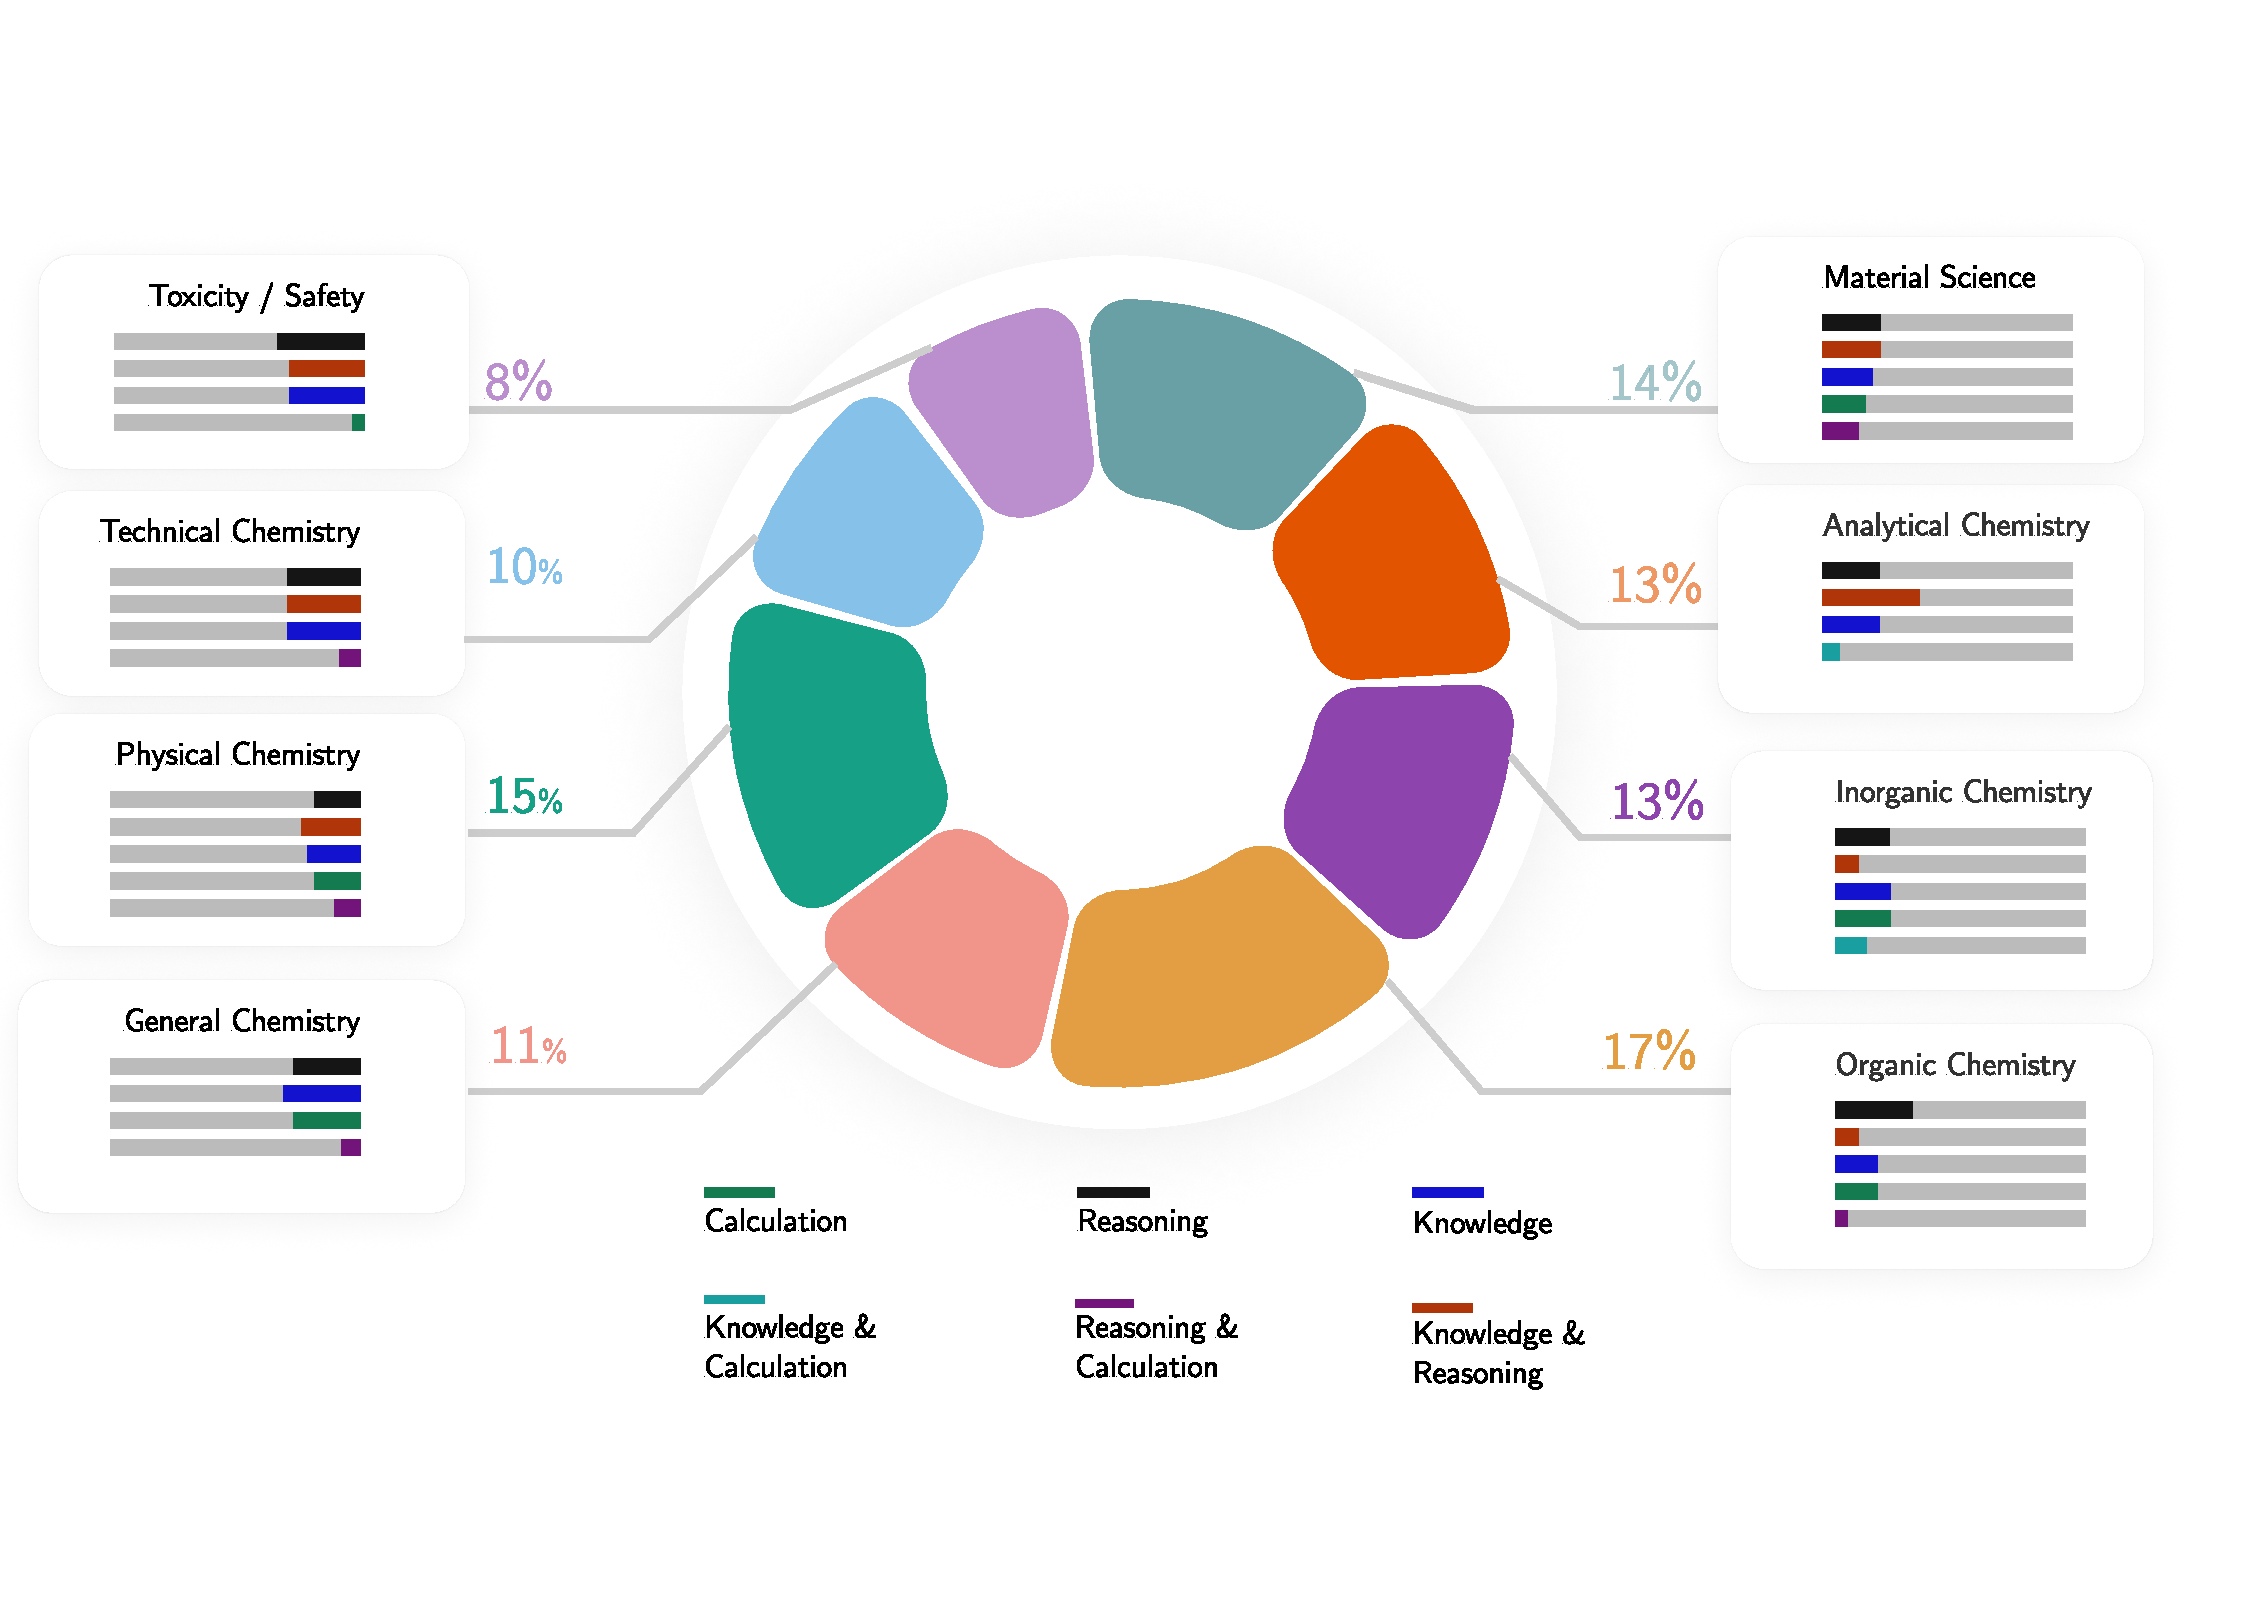
\includegraphics[width=\textwidth]{figures/CB_HUMANSET_FIG_V1.pdf}
    \caption{\textbf{Composition of the human subset.} The circular plot shows the distribution of topics and required skills in the human subset of the \chembench corpus. The human subset is a representative subset of the full corpus, with a balanced distribution of topics and skills.}
    \label{fig:cb_humanset}
\end{figure}

The corpus of the questions in \chembench, as shown in \Cref{tab:chembench_corpus_topic}, can be divided according to which chemical topic they belong to.

%\begin{table}
%    \centering
%    \small
%    \caption{\textbf{Examples for each of the topics considered in the evaluation of the \chembench corpus.} The table shows the percentage of questions in the corpus that belong to each topic, as well as example questions.}
%    \label{tab:chembench_corpus_topic}
%    {\fontsize{8}{9}\selectfont
%        \begin{tabularx}{\textwidth}{X}
%            \toprule
%            \multicolumn{1}{c}{\textbf{Analytical Chemistry} 166 Questions (5.8\%)} \\
%            \midrule
%            Which of the following analytical methods is most appropriate for performing a survey analysis of a solid sample containing various metals? \\
%            A. X-ray fluorescence analysis \\
%            B. Differential pulse polarography \\
%            C. Flame-atomic absorption spectroscopy \\
%            D. Gas chromatography with flame ionization detector \\
%            E. Hydride generation atomic absorption spectroscopy \\
%            \midrule
%            \multicolumn{1}{c}{\textbf{Chemical Preference} 1001 Questions (35\%)} \\
%            \midrule
%            Imagine an early virtual screening campaign setting (accounting for simple aspects such as oral availability and small molecular profile, but no other modalities such as covalency or bifunctionality). Which of the following two candidates would you prefer for further development? \\
%            [START\_SMILES]N\#Cc1ccc(OCCCN2CC3CN\-(CCNS(=O)(=O)c4ccc(F)cc4)CC(C2)O3)cc1\-[END\-\_SMILES] \\
%            [START\_SMILES]O=C1CC(c2ccc(CC(NS(=O)\-(=O)\-c3cc(Cl)cc(Cl)c3)c3nc4ccccc4[nH]3)cc2)S\-(=O)\-(=O)N1[END\_SMILES] \\
%            \midrule
%            \multicolumn{1}{c}{\textbf{General Chemistry} 152 Questions (5.3\%)} \\
%            \midrule
%            Which of the following salts is an acidic salt? \\
%            A. \ce{NH4Cl} \\
%            B. \ce{Na2CO3} \\
%            C. \ce{NaH2PO4} \\
%            D. \ce{Zn(OH)Cl} \\
%            \midrule
%            \multicolumn{1}{c}{\textbf{Inorganic Chemistry} 94 Questions (3.3\%)} \\
%            \midrule
%            What is the oxidation number of the metal in the compound \ce{[ZrF7]^{3-}}\\
%            \midrule
%            \multicolumn{1}{c}{\textbf{Materials Science} 89 Questions (3.1\%)} \\
%            \midrule
%            For NMR analysis, you need to digest the MOF in a strong acid to remove the linker and leave the metal clusters intact. Why would one choose \ce{HF} over \ce{HCl} for this purpose? \\
%            A. \ce{F-} forms a stable bonds to the metal ions \\
%            B. \ce{HF} has a better water solubility than \ce{HCl} \\
%            C. \ce{HF} has a higher boiling point than \ce{HCl} \\
%            D. \ce{HF} is a weaker acid than \ce{HCl} \\
%            \midrule
%            \multicolumn{1}{c}{\textbf{Organic Chemistry} 441 Questions (15.5\%)} \\
%            \midrule
%            What is the reaction mechanism that describes the following reaction (represented using reaction SMILES) [START\_RXNSMILES]CCCl.CO[Na]>>[Na]Cl.CCOC\-[END\_RXNSMILES]? \\
%            A. $E_1$ \\
%            B. $E_{cb}$ \\
%            C. $S_N1$ \\
%            D. $S_N2$ \\
%            \midrule
%            \multicolumn{1}{c}{\textbf{Physical Chemistry} 179 Questions (6.3\%)} \\
%            \midrule
%            The Born-Oppenheimer (BO) approximation is widely used in computational chemistry, but its accuracy can vary depending on the system. Among the following options, for which system is the Born-Oppenheimer approximation likely to be least applicable? \\
%            A. \ce{C60} \\
%            B. \ce{CH4} \\
%            C. \ce{Fe(CO)5} \\
%            D. \ce{H2+} \\
%            E. \ce{NaCl} \\
%            \midrule
%            \multicolumn{1}{c}{\textbf{Technical Chemistry} 42 Questions (1.5\%)} \\
%            \midrule
%            Which of the following statements is true about the different types of ideal reactors? \\
%            A. In a batch reactor, the composition is uniformly mixed and remains the same throughout the reactor and at the exit \\
%            B. In a batch reactor, the fluid passes through the reactor with no mixing of earlier and later entering fluid \\
%            C. In a mixed flow reactor, the composition changes with time but is uniform everywhere within the reactor \\
%            D. In a plug flow reactor, the fluid moves in single flow through the reactor with no mixing and no overtaking \\
%            \midrule
%            \multicolumn{1}{c}{\textbf{Toxicity/Safety} 690 Questions (24.2\%)} \\
%            \midrule
%            Pindolol and propranolol are (relatively nonselective) antagonists at $\beta_1$- and $\beta_2$-adrenoceptors. However, pindolol is a partial agonist, whereas propranolol is a pure antagonist. What follows from this? \\
%            A. Pindolol has a greater therapeutic range than propranolol \\
%            B. Pindolol has a longer half-life than propranolol \\
%            C. Pindolol has intrinsic activity \\
%            D. Pindolol is more lipophilic than propranolol \\
%            E. Pindolol is more potent than propranolol \\
%            \bottomrule
%        \end{tabularx}
%    }
%\end{table}

\normalsize


In addition, as shown in \Cref{tab:cb_skillset} the \chembench corpus can be divided considering the different skills needed to solve the questions. The plot shows a balanced distribution of the required skills in the \chembench corpus. \Cref{tab:cb_skillset} shows an example question for each skill category.

\begin{figure}
    \centering
    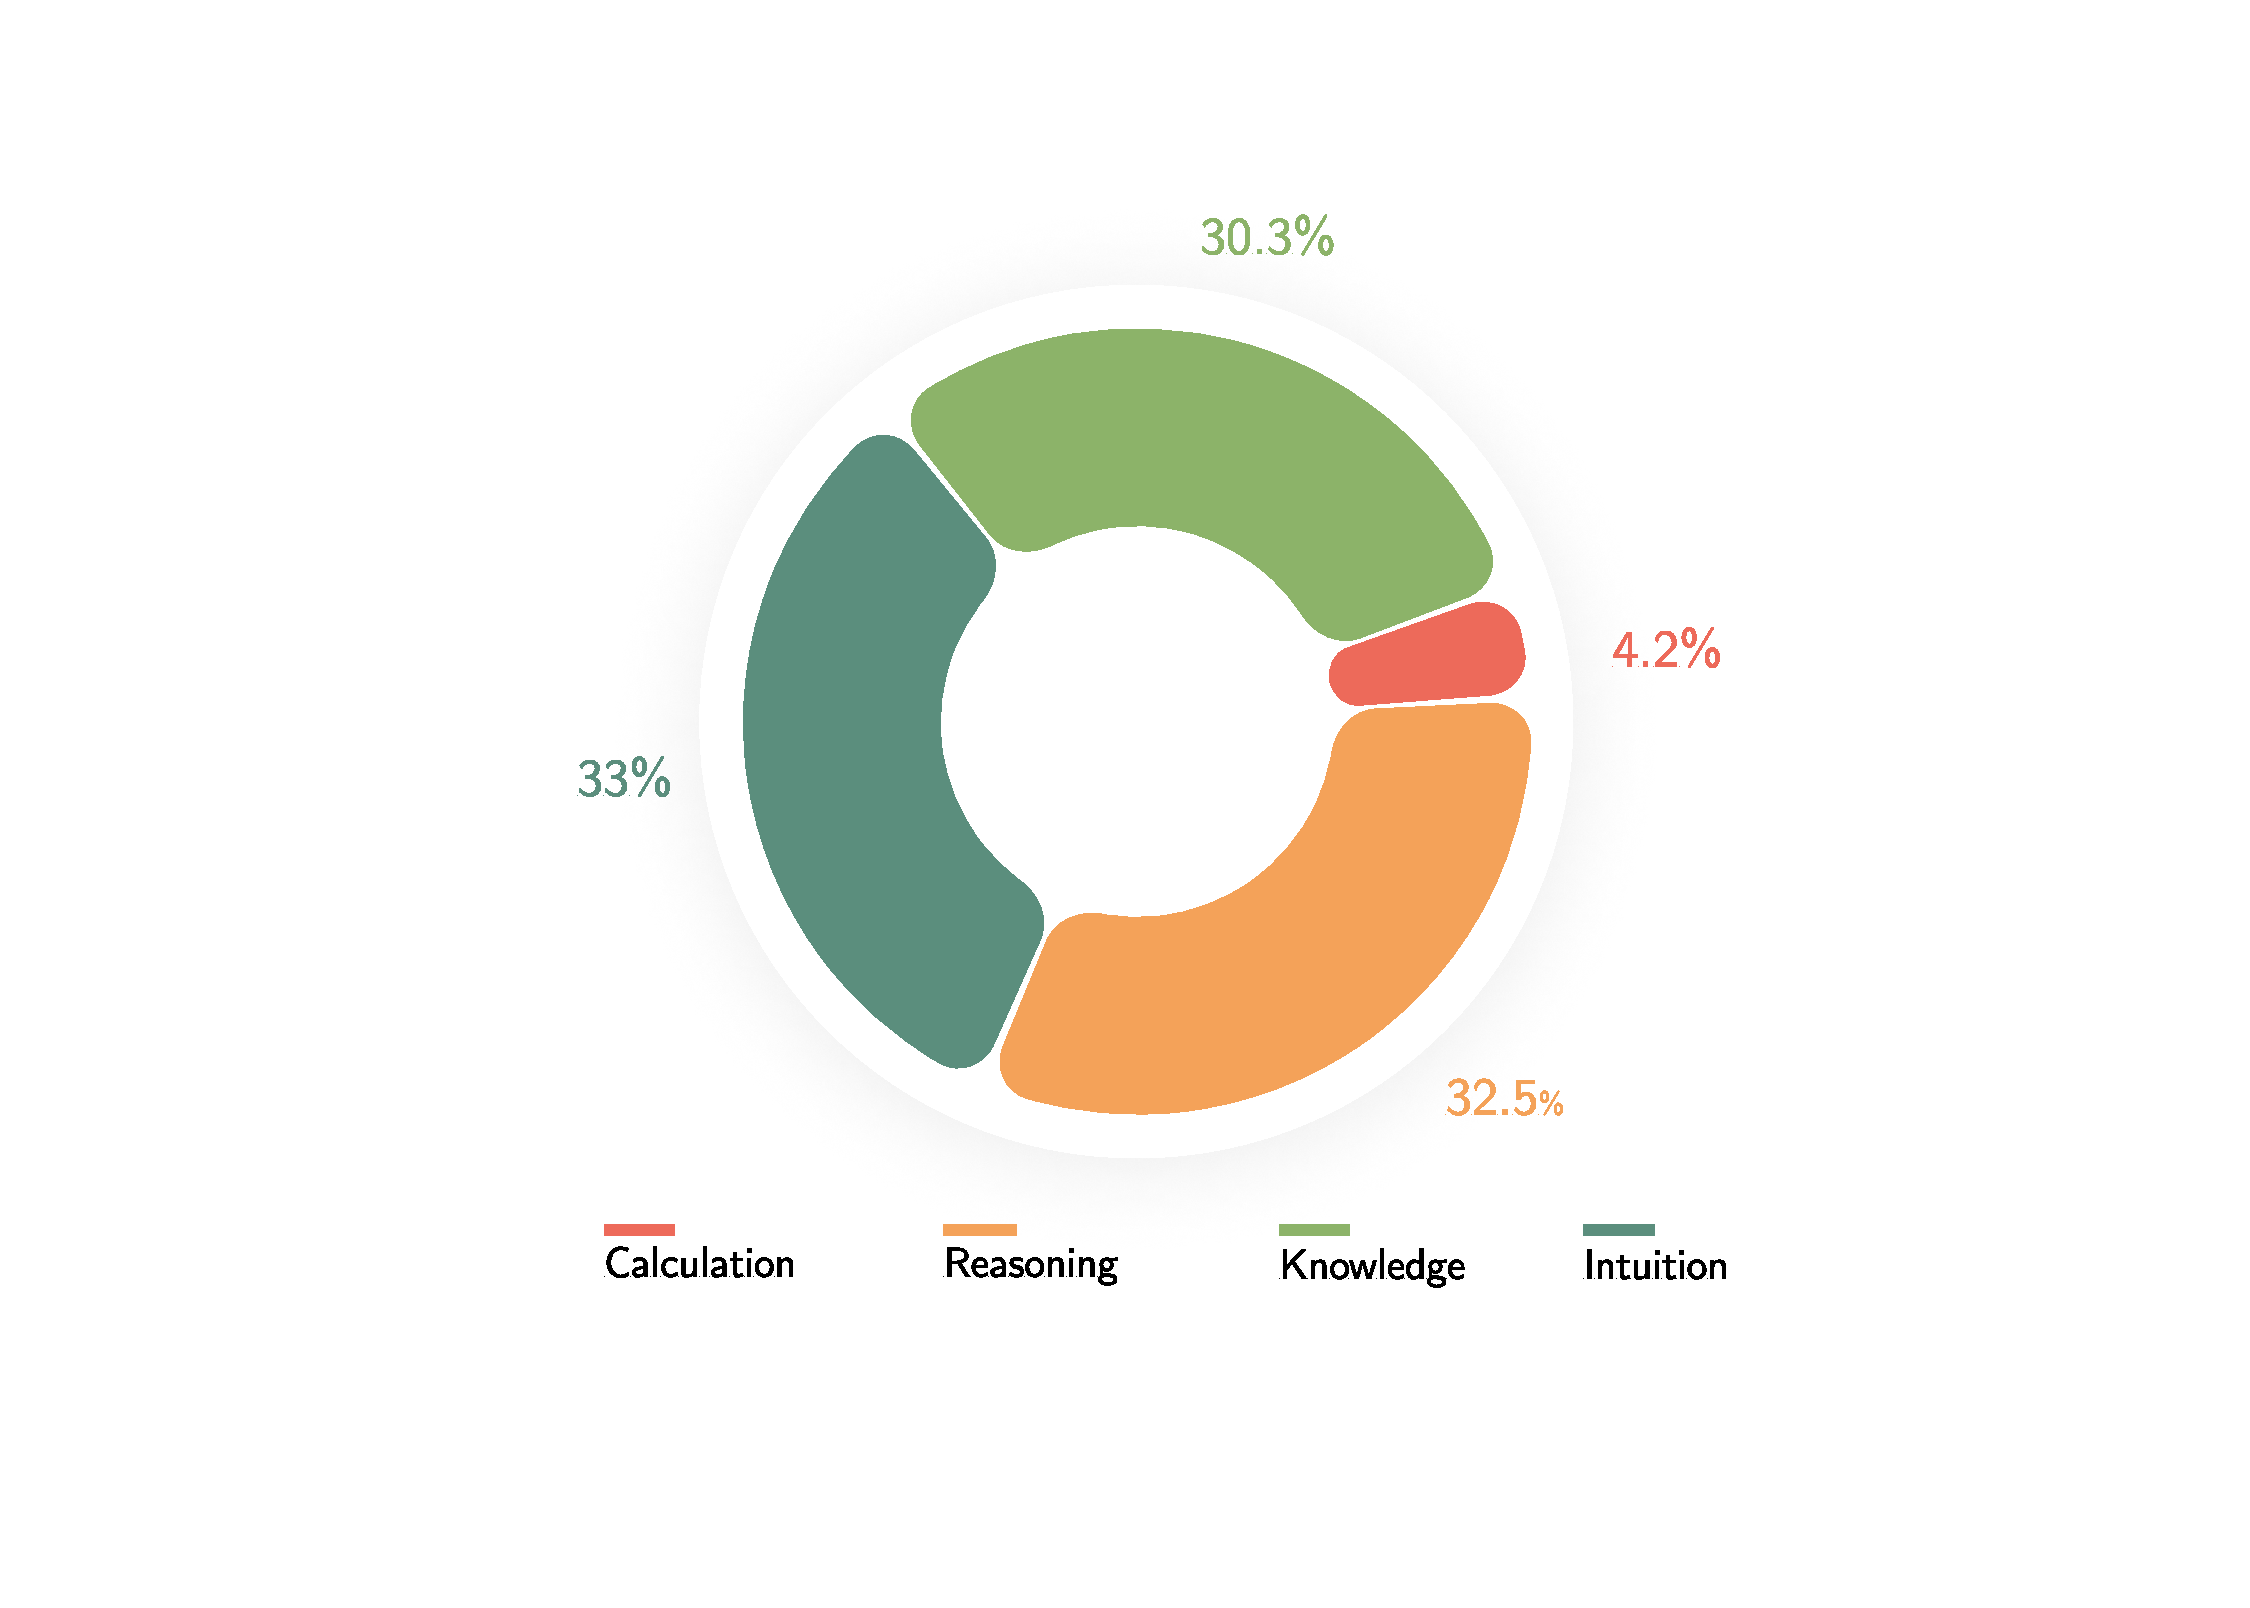
\includegraphics[width=\textwidth]{figures/CB_SKILL_FIG_V1.pdf}
    \caption{\textbf{Composition of the required skills considered in the \chembench corpus.} The circular plot shows the distribution of required skills in the \chembench corpus.}
    \label{fig:cb_skillset}
\end{figure}


\begin{table}
    \centering
    \small
    \caption{\textbf{Examples for each of the required skills considered in the \chembench corpus.} The table shows the number of questions for each skill and an example question. Note that the total count in this table is bigger than the \chembench corpus. This is because the same question can be annotated with two different \enquote{requires} skills, i.e. Reasoning and Calculation.}
    \label{tab:chembench_corpus_cognitive}
    {\fontsize{8}{9}\selectfont
        \begin{tabularx}{\textwidth}{X}
            \toprule
            \multicolumn{1}{c}{\textbf{Knowledge} 919 Questions} \\
            \midrule
            Which of the following salts is an acidic salt? \\
            A. \ce{NH4Cl} \\
            B. \ce{Na2CO3} \\
            C. \ce{NaH2PO4} \\
            D. \ce{Zn(OH)Cl} \\
            \midrule
            \multicolumn{1}{c}{\textbf{Reasoning} 987 Questions} \\
            \midrule
            How can the optical impact of quantum confinement on the electronic structure of a quantum dot be observed experimentally? \\
            A. By atomic force microscopy \\
            B. By transform infrared spectroscopy \\
            C. By measuring a photoluminescence spectrum \\
            D. By absorption spectroscopy \\
            \midrule
            \multicolumn{1}{c}{\textbf{Intuition} 1001 Questions} \\
            \midrule
            Imagine an early virtual screening campaign setting (accounting for simple aspects such as oral availability and small molecular profile, but no other modalities such as covalency or bifunctionality). Which of the following two candidates would you prefer for further development? \\
            A. [START\_SMILES]CC1(C)Oc2ccc([N+](=O)[O-])cc2[C@@H](N2CCOCC2)[C\@\@H]1O[END\_SMILES] \\
            B. [START\_SMILES]Cc1ccccc1N=C(S)N1CCC(NC\-(=O)c2ccco2)CC1[END\_SMILES] \\
            \midrule
            \multicolumn{1}{c}{\textbf{Calculation} 128 Questions} \\
            \midrule
            Given that the average molar mass of the polymer chains in this sample of poly(lactic acid) (PLA) is \SI{595}{g mol^{-1}} using end-group analysis, where \SI{0.1619}{g} of PLA was dissolved in \SI{25}{cm^3} of benzyl alcohol and titrated with \SI{0.0400}{mol dm^{-3}} \ce{KOH} solution. The volume of \ce{KOH} solution required to reach the endpoint was \SI{6.81}{cm^3}. What is the average number of monomer units in each polymer chain of this sample? \\
            \bottomrule
        \end{tabularx}
    }
\end{table}

\normalsize

In analyzing the performance of state-of-the-art models on the ChemBench corpus, we identified several chemical topics where the models consistently struggled to provide correct answers. The following table \cref{tab:chembench_corpus_models_failed_topic} presents examples of challenging questions across different chemical domains, highlighting specific areas where current models need improvement

%\begin{table}
%    \centering
%    \small
%    \caption{\textbf{Examples of topics evaluated in the \chembench corpus that the state-of-the-art model failed to answer correctly.} The table displays the percentage of questions in the corpus for each topic, along with example questions and the percentage of questions that were not answered correctly by the models.}
%    \label{tab:chembench_corpus_models_failed_topic}
%    {\fontsize{8}{9}\selectfont
%        \begin{tabularx}{\textwidth}{X}
%            \toprule
%            \multicolumn{1}{c}{\textbf{Analytical Questions} 166 Questions (5.8\%) (26.5\%)} \\
%            \midrule
%            Which of the following methods can be used to support the structure elucidation of planar molecules by examining the topography of individual molecules? \\
%            A. DESI-mass spectrometry \\
%            B. XPS \\
%            C. atomic force microscopy \\
%            D. scanning tunneling microscopy \\
%            E. secondary ion mass spectrometry \\
%            \midrule
%            \multicolumn{1}{c}{\textbf{Chemical Preference} 1001 Questions (35\%) (8.5\%)} \\
%            \midrule
%            Imagine an early virtual screening campaign setting (accounting for simple aspects such as oral availability and small molecular profile, but no other modalities such as covalency or bifunctionality). Which of the following two candidates would you prefer for further development? \\
%            [START\_SMILES]N\#Cc1ccc(OCCCN2CC3CN\-(CCNS(=O)(=O)c4ccc(F)cc4)CC(C2)O3)cc1\-[END\-\_SMILES] \\
%            [START\_SMILES]O=C1CC(c2ccc(CC(NS(=O)\-(=O)\-c3cc(Cl)cc(Cl)c3)c3nc4ccccc4[nH]3)cc2)S\-(=O)\-(=O)N1[END\_SMILES] \\
%            \midrule
%            \multicolumn{1}{c}{\textbf{General Chemistry} 152 Questions (5.3\%) (3.2\%)} \\
%            \midrule
%            Why \ce{SCl6} does not exist if other similar molecules such as \ce{SF6} exist? \\
%            A. \ce{SCl6} does not exist because of steric effects \\
%            B. \ce{SCl6} does not exist because of the high electronegativity of chlorine \\
%            C. \ce{SCl6} does not exist because of the high ionization potential of the chlorine \\
%            D. \ce{SF6} exist because of the high electronegativity of fluorine \\
%            \midrule
%            \multicolumn{1}{c}{\textbf{Inorganic Chemistry} 94 Questions (3.3\%) (4.2\%)} \\
%            \midrule
%            What is the spin-only magnetic moment (in units of Bohr-magnetons) for the low-spin case of the metal complex \ce{RhCl(CO)(PPh3)2}?\\
%            \midrule
%            \multicolumn{1}{c}{\textbf{Materials Science} 89 Questions (3.1\%) (0.9\%)} \\
%            \midrule
%            What are the conditions for the observation of effects of quantum confinement in quantum dots? \\
%            A. All dimension of the material must be smaller than exciton Bohr radius \\
%            B. One dimension of the quantum dot must be smaller than exciton Bohr radius \\
%            C. The movement od charge carriers is limited in all spatial dimensions \\
%            \midrule
%            \multicolumn{1}{c}{\textbf{Organic Chemistry} 441 Questions (15.5\%) (0.5\%)} \\
%            \midrule
%            What makes acrylates more reactive than typical hydrocarbons? \\
%            A. The carbonyl group \\
%            B. The double bond \\
%            C. The hydroxyl group \\
%            D. The vinyl group \\
%            \midrule
%            \multicolumn{1}{c}{\textbf{Physical Chemistry} 179 Questions (6.3\%) (13.4\%)} \\
%            \midrule
%            Why are polar molecules more soluble in water than non-polar molecules? \\
%            A. Non-polar molecules should break hydrogen bonds in water to dissolve \\
%            B. The entropy of the system increases when non-polar molecules dissolve in water \\
%            C. Water has a dipole and can easier isolate polar molecules from each other \\
%            D. Water makes stable dipole-dipole interactions with polar molecules \\
%            \midrule
%            \multicolumn{1}{c}{\textbf{Technical Chemistry} 42 Questions (1.5\%) (4.7\%)} \\
%            \midrule
%            Which of the following statements is/are true about granulation shaping of solid catalysts? \\
%            A. Broader product diameter distribution than pellets or extrudates \\
%            B. Facilitates reactor upscaling \\
%            C. It is also called snow-ball \\
%            D. Not suitable to prepare egg-shell catalysts \\
%            \midrule
%            \multicolumn{1}{c}{\textbf{Toxicity/Safety} 690 Questions (24.2\%) (40.4\%)} \\
%            \midrule
%            What determines the flammability of polyols? \\
%            A. Their chemical structure \\
%            B. Their low volatility \\
%            C. Their odor threshold \\
%            D. Their reaction with acids \\
%            \bottomrule
%        \end{tabularx}
%    }
%\end{table}

\normalsize

To better understand the cognitive demands of chemical assessment, we categorized the questions in the ChemBench corpus according to the primary skills required to solve them. The table \Cref{tab:chembench_corpus_models_failed_cognitive} below shows representative examples of questions that state-of-the-art models failed to answer correctly across different cognitive skill categories, including knowledge, reasoning and intuition.
\begin{table}
    \centering
    \small
    \caption{\textbf{Examples of required skills evaluated in the \chembench corpus that the state-of-the-art model failed to answer correctly} The table displays the number of questions for each skill, along with an example question that the model failed to answer.}
    \label{tab:chembench_corpus_models_failed_cognitive}
    {\fontsize{8}{9}\selectfont
        \begin{tabularx}{\textwidth}{X}
            \toprule
            \multicolumn{1}{c}{\textbf{Knowledge} 919 Questions} \\
            \midrule
            Which of the following are true for phosphoric acid? \\
            A. Is a weak acid, so it is not toxic \\
            B. Should never be tasted \\
            C. Though a component of soft drinks, reacts vigorously with water when in concentrated form \\
            \midrule
            \multicolumn{1}{c}{\textbf{Reasoning} 987 Questions} \\
            \midrule
            Which of the following elements has the largest atomic radius? \\
            A. \ce{Fr} \\
            B. \ce{He} \\
            C. \ce{Li} \\
            D. \ce{Rb} \\
            \midrule
            \multicolumn{1}{c}{\textbf{Intuition} 1001 Questions} \\
            \midrule
            Imagine an early virtual screening campaign setting (accounting for simple aspects such as oral availability and small molecular profile, but no other modalities such as covalency or bifunctionality). Which of the following two candidates would you prefer for further development? \\
            A. [START_SMILES]CCc1c(CCOC)nn(-c2ccccc2)c1-c1ccccc1[END_SMILES] \\
            B. [START_SMILES]Cc1cc(/C=C2\\C(=N)N3N=C(S(C)(=O)=O)SC3=NC2=O)c(C)n1Cc1ccccc1[END_SMILES] \\
            \midrule
            \multicolumn{1}{c}{\textbf{Calculation} 128 Questions} \\
            \midrule
            The cell potential for the overall cell reaction during electrolysis of water, \ce{2H2O(l) -> 2H2(g) + O2(g)} is \SI{-1.23 V}. What is the standard electrode potential for the half reaction, \ce{2H2O(l) -> O2(g) + 4H+(aq) + 4e-} in V? \\
            \bottomrule
        \end{tabularx}
    }
\end{table}

\normalsize




\clearpage
\subsection{Model performance} \label{sec:model_performance_app}
We also evaluated the model performance on the entire \chembench corpus.
\Cref{fig:barplot_all_correct_all_questions} shows the fraction of questions that were answered correctly by the models.

\begin{figure}[htb]
    \centering
    \includegraphics{figures/overall_performance.pdf}
    \caption{\textbf{Overall performance of the models on the \chembench corpus.} The bar plot shows the fraction of questions that were answered completely correctly by the models. Scores computed on the entire \chembench corpus.}
    \label{fig:barplot_all_correct_all_questions}
    \script{plot_overview_performance_plot.py}
\end{figure}

\Cref{fig:all_questions_models_completely_correct_radar_overall} shows the performance of the models on the different topics of the \chembench corpus.
The general pattern of performance varies significantly between the different topics and is also observed when the models are evaluated on the entire corpus.
However, since some subjects are composed of questions from different sources, the ranking of the models is, in some instances, different from the one on \chembenchmini.

\begin{figure}[htb]
    \centering
    \includegraphics[width=\textwidth]{figures/all_questions_models_completely_correct_radar_overall.pdf}
    \caption{\textbf{Performance of the models on the different topics of the \chembench corpus.} The radar plot shows the performance of the models on the different topics of the \chembench corpus. The performance is measured as the fraction of questions answered completely correctly by the models.
    A score of 1 (full coverage until the outer line of this plot) indicates that all questions were answered completely correctly, while a score of 0 indicates that none were answered completely correctly.
    }
    \label{fig:all_questions_models_completely_correct_radar_overall}
    \script{analyze_model_reports.py}
\end{figure}




To further investigate the performance of the models, we also compared the performance on different data sources.
Compared to topics, this is a more fine-grained analysis, as topics can be composed of questions from different sources.
In \Cref{fig:performance_per_topic}, we see that the performance of the models varies significantly between the different data sources.
Interestingly, the performance of the models on questions sourced based on textbooks seems to be better for our models than some semi-programmatically created tasks, such as questions about the number of signals in an \gls{nmr} spectrum.


\begin{figure}[htb]
    \centering
    \includegraphics{figures/performance_per_topic.pdf}
    \caption{\textbf{Fraction of correctly answered questions per data source.} The heatmap shows, in color, the fraction of questions answered correctly by different systems for some of our data sources. The performance is measured as the fraction of questions answered completely correctly by the models. A score of one (red) indicates that all questions were answered completely correctly, while a score of zero (blue) indicates that none of the questions were answered completely correctly.
        We see that the performance of the models varies significantly between the different data sources. For instance, it is interesting to observe that questions sourced based on textbooks seem easier for our leading models than for humans. However, this performance does not correlate with performance on other sources, e.g., semi-programmatically created tasks such as questions about the number of signals in an \gls{nmr} spectrum.
    }
    \label{fig:performance_per_topic}
    \script{analyze_performance_per_source.py}
\end{figure}

\Cref{fig:performance_per_topic_tiny} shows the same analysis on \chembenchmini.

\Cref{fig:performance_corpus_and_tiny} shows the performance of the models on the \chembench corpus and the \chembenchmini subset. The relative performance difference between both is quite similar across most models.
This makes \chembenchmini subset a reliable subset for human baseline comparison and particularly valuable for rapid prototyping and initial model assessment phases.

An interesting observation is the significant impact of chemical preference tasks on \GPTFour's scores. A detailed breakdown of overall accuracy into scores on different skills and difficulty levels is provided in \Cref{table:performance_table} and \Cref{tab:performance_table_human_subset} for \chembench corpus and the \chembenchmini subset, respectively.


\begin{figure}[htb]
    \centering
    \includegraphics{figures/performance_per_topic_tiny.pdf}
    \caption{\textbf{Fraction of  correctly answered questions per data source on \chembenchmini.} The heatmap shows, in color, the fraction of questions answered completely correctly by different systems for some of our data sources. The performance is measured as the fraction of questions answered completely correctly by the models. A score of one (red) indicates that all questions were answered completely correctly, while a score of zero (blue) indicates that none were answered completely correctly.
        We see that the performance of the models varies significantly between the different data sources. For instance, it is interesting to observe that questions sourced based on textbooks seem easier for the leading models than for humans. However, this performance does not correlate with performance on other sources, e.g., semi-programmatically created tasks such as questions about the number of signals in an \gls{nmr} spectrum.
    }
    \label{fig:performance_per_topic_tiny}
    \script{analyze_performance_per_source.py}
\end{figure}


\begin{figure}[htb]
    \centering
    \includegraphics{figures/corpus_human_comparison.pdf}
    \caption{\textbf{
        Performance of the models on the \chembench corpus and \chembenchmini subset.} The bar plot shows the fraction of questions that were answered completely correctly, highlighting the relative performance of different models on both the \chembench corpus and the \chembenchmini subset.
        We see that the model ranking remains fairly consistent across both sets}
    \label{fig:performance_corpus_and_tiny}
    \script{corpus_humanset_performance.py}
\end{figure}

\begin{table}
    \caption{\textbf{Performance of the models on the \chembench corpus.} The table shows the fraction of questions answered completely correctly by the models for different skills and difficulty levels.}
    \resizebox{\textwidth}{!}{
    \variable{output/performance_table.tex}
    }
    \label{tab:performance_table}
\end{table}

\begin{table}
    \caption{\textbf{Performance of the models on \chembenchmini.} The table shows the fraction of questions answered completely correctly by the models for different skills and difficulty levels.}
    \resizebox{\textwidth}{!}{
    \variable{output/performance_table_human_subset.tex}
    }
    \label{tab:performance_table_human_subset}
\end{table}



\clearpage

\subsection{Performance as a function of molecular features} \label{sec:molecular_features}
To better understand if the performance of the models is correlated with specific features of the molecules, we analyzed the performance of the models as a function of the number of atoms and the complexity of the molecules.
\Cref{fig:correlation_plot_is_number_nmr_peaks_complexity} shows that the performance of the models is not correlated with the complexity of the molecules but rather with the number of atoms (\Cref{fig:correlation_plot_is_number_nmr_peaks_num_atoms}, similar trivial correlation for \Cref{fig:correlation_plot_is_electron_counts_num_atoms}).
%The corresponding Spearman correlation coefficients are listed in \Cref{tab:correlation_coefficients}.

\begin{figure}[!h]
    \centering
    \includegraphics[width=\textwidth]{figures/correlation_plot_is_number_nmr_peaks_complexity.pdf}
    \caption{\textbf{Dependence of the mean absolute error in predicting the number of NMR signals on the Böttcher complexity of the molecules.} The complexity measure proposed by \textcite{B_ttcher_2016} is an information-theoretic additive measure of compound complexity that follows chemical intuitions.
    The plot shows that for the \glspl{llm}, the predictive performance (measured as the mean absolute error in the prediction of the number of \gls{nmr} signals) is not correlated with the complexity of the molecules (that is, molecules tend to not to be able to predict the number of \gls{nmr} signals irregardless of molecular complexity). For inference based on reasoning, one would expect that the complexity of the molecule is a good predictor of the difficulty of the question.}
    \script{correlate_with_molecule_features.py}
    \label{fig:correlation_plot_is_number_nmr_peaks_complexity}
\end{figure}

\begin{figure}[!h]
    \centering
    \includegraphics[width=\textwidth]{figures/correlation_plot_is_number_nmr_peaks_num_atoms.pdf}
    \caption{\textbf{Dependence of the mean absolute error in predicting the number of NMR signals on the number of atoms.} }
    \script{correlate_with_molecule_features.py}
    \label{fig:correlation_plot_is_number_nmr_peaks_num_atoms}
\end{figure}


\begin{figure}[!h]
    \centering
    \includegraphics[width=\textwidth]{figures/correlation_plot_is_electron_counts_num_atoms.pdf}
    \caption{\textbf{Dependence of the mean absolute error in predicting total electron counts on the number of atoms.} The plot shows that for the \glspl{llm}, the predictive performance (measured as the mean absolute error in the prediction of the total electron counts) is sometimes correlated with the number of atoms in the molecule.}
    \script{correlate_with_molecule_features.py}
    \label{fig:correlation_plot_is_electron_counts_num_atoms}
\end{figure}


\clearpage
\subsection{Influence of model scale}
\Cref{fig:model_size_plot} shows the performance of the models as a function of the number of parameters in the model.
We see that the performance of the models correlates with their size for the models of the LLama-3 and Llama-3.1 herd of models.

\begin{figure}[!h]
    \centering
    \includegraphics[width=\textwidth]{figures/model_size_plot.pdf}
    \caption{\textbf{Performance of models as a function of model size.} The plot shows the performance of the models as a function of the parameter count. The performance is measured as the fraction of questions answered correctly by the models. We see that the performance of the models correlates with scale for the models of the LLama-3 and Llama-3.1 herd of models.}
    \script{performance_vs_model_size.py}
    \label{fig:model_size_plot}
\end{figure}


\clearpage
\subsection{Refusal detection}
\Glspl{llm} typically undergo refusal training to prevent harmful or undesirable outputs. As a result, models may decline to answer questions perceived as potentially adversarial prompts.
To automatically detect refusals, we use a modified regular expression reported by LLM Guard\autocite{llmguard} to detect commonly used refusal phrases.

\Cref{tab:refusal_counts_and_parsing} lists how many refusals were detected for the reponses of different models on \chembench. Overall, we find that refusals do not majorly affect the performance measured by \chembench.


\subsection{LLM Parsing} \label{sec:llm-parsing}

In our parsing workflow, we use pipelines based on regular expressions to extract the answers. In some cases, however, the answers are not directly extractable from the responses, for instance, when the model does not follow the formatting instructions. In these cases, we use a fallback mechanism to extract the answers. The fallback mechanism uses an \gls{llm} to extract the answers from the responses. The \gls{llm} is provided with the response and the question and is prompted to only extract but not generate the answer. We used \LlamaThreeSeventyBInstruct, accessed via the Groq API.
\Cref{tab:refusal_counts_and_parsing} tabulates the number of times the fallback mechanism was used for each model.


\begin{table}
    \centering
    \caption{\textbf{Refusal counts and parsing.} The table shows the number of refusals detected and the number of times the \gls{llm} fallback parsing mechanism was used for each model.}
    \variable{output/model_refusal_table.tex}
    \label{tab:refusal_counts_and_parsing}
\end{table}

\clearpage
\subsection{Implementation}
An overview of the benchmarking pipeline implemented in \chembench is shown in \Cref{fig:process}. More detailed information can be found in the online documentation of the \chembench package at \url{https://lamalab-org.github.io/chem-bench/}.
\begin{figure}
    \centering
    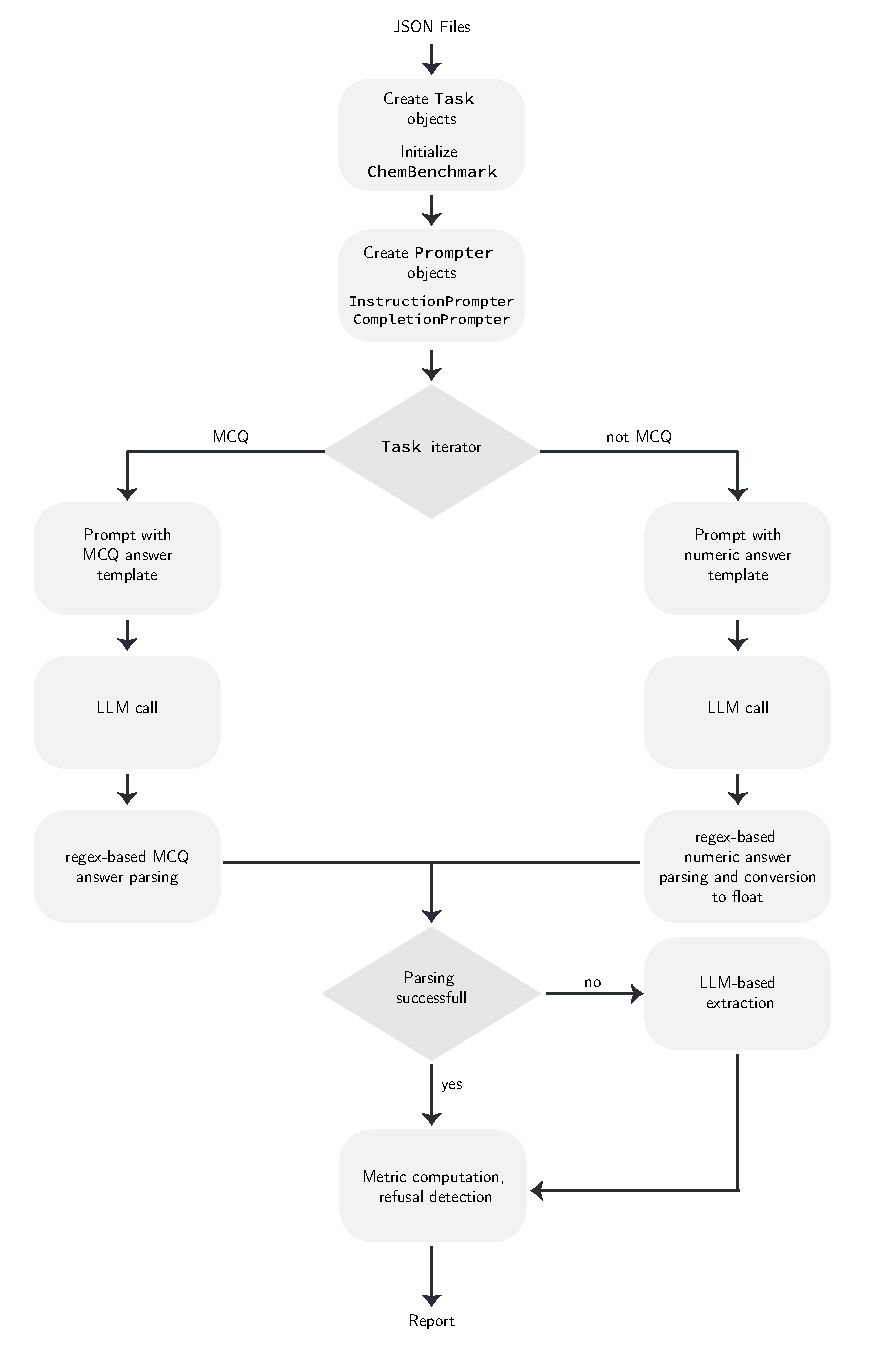
\includegraphics[height=.7\textheight]{figures/process.pdf}
    \caption{\textbf{Overview of the benchmarking pipeline implemented in \chembench.} The process begins with JSON files containing task data, which are used to create \texttt{Task} objects and initialize the \texttt{ChemBenchmark}. \texttt{Prompter} objects are then created to handle different types of prompts for instruction-tuned and completion models.
    The \texttt{Task} Iterator differentiates between \gls{mcq} and other question types. For each task type, appropriate prompts are generated and passed to the \gls{llm}. The responses are then processed using regex-based parsing methods specific to \gls{mcq} or numeric answers (after obtaining the relevant part of the response from the instruction-tuned models).
    The regex-based parsing is elaborate and also able to handle special cases such as scientific notation, or roman numerals.
    If the initial parsing is unsuccessful, the system employs an \gls{llm}-based extraction method as a fallback. The parsed or extracted answers then undergo metric computation and refusal detection.}
    \label{fig:process}
\end{figure}



\clearpage
\subsection{Human baseline} \label{sec:human_baseline}
\paragraph{App} To facilitate the collection of responses, we developed a responsive web application in Typescript using the Next.js\autocite{nextjs} app router framework.
This application handles serving the user interface and exposes various \gls{rest} \glspl{api} for relevant operations.
We utilize a Postgresql.
The web application is styled with Tailwind CSS\autocite{tailwindcss} using the shadcn/ui component library and uses NextAuth\autocite{nextauth} for easy and secure user authentication.
The application is hosted on the Vercel web hosting platform.

In the applications, human participants were presented with molecules as rendered drawings and SMILES strings. \LaTeX\xspace equations and chemical equations were rendered using MathJax (\Cref{fig:screenshots}).


\begin{figure}
    \subfloat[A physcial chemistry question.]{
        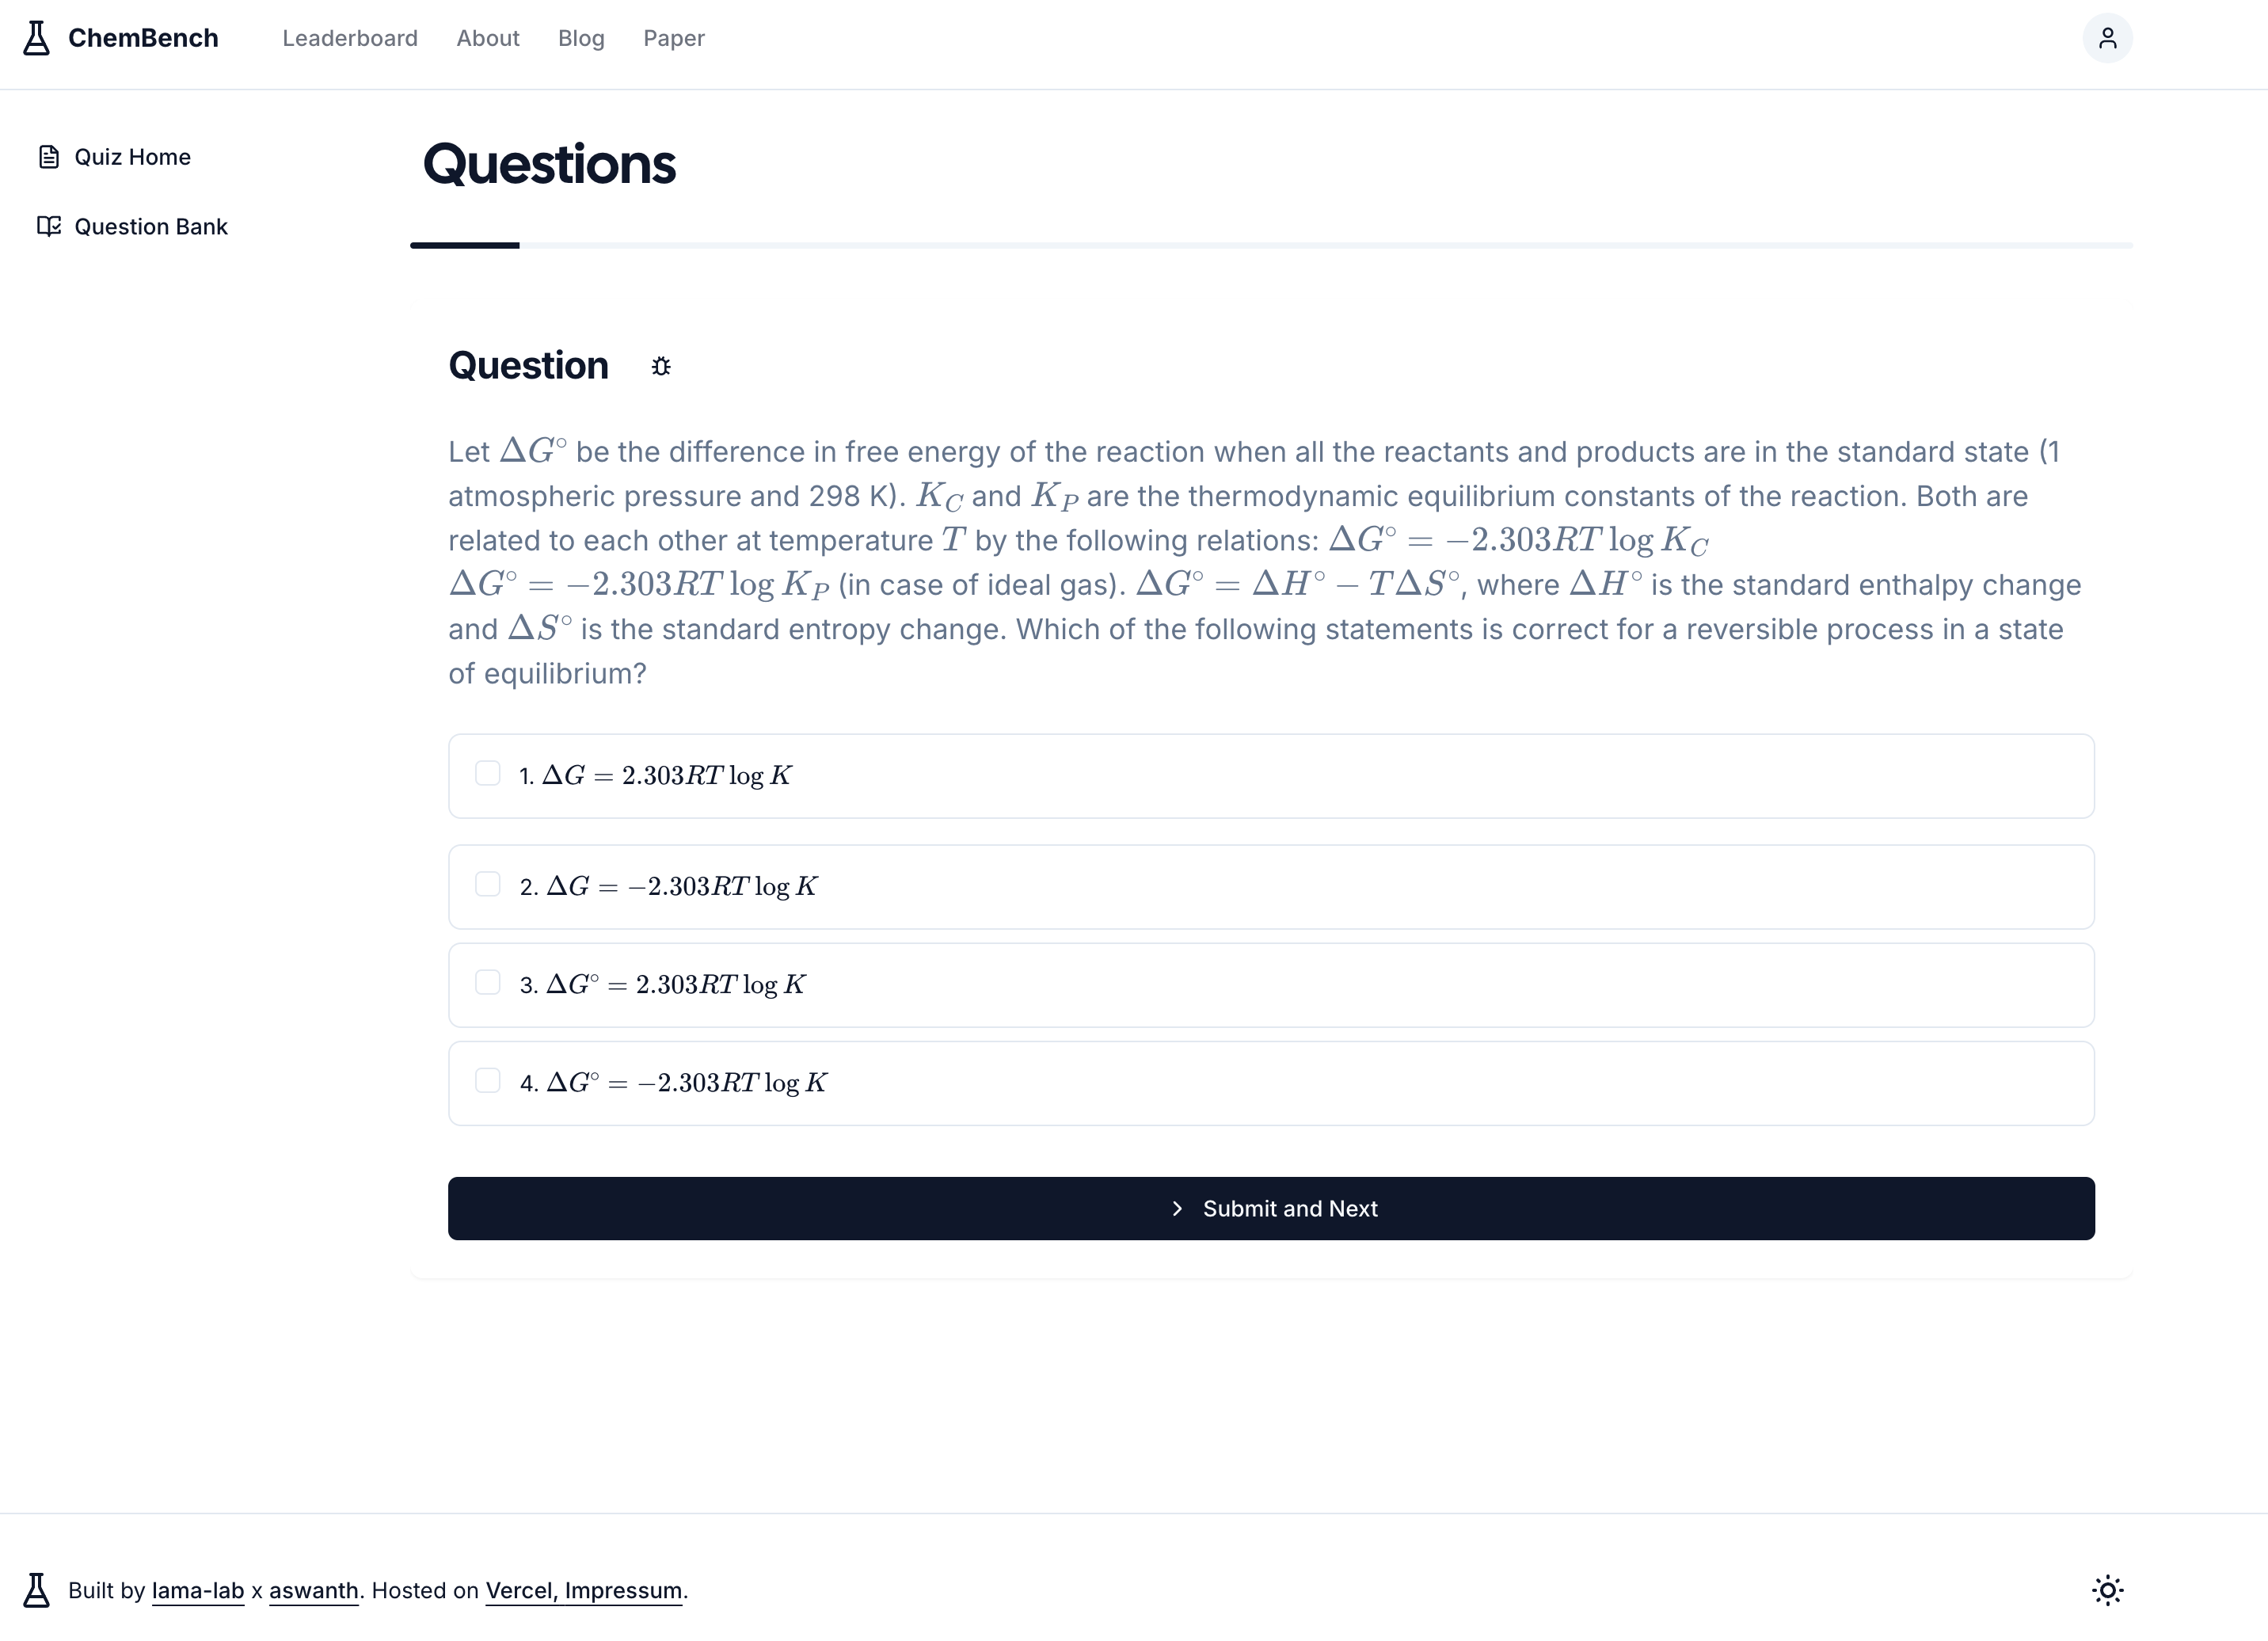
\includegraphics[width=\textwidth]{figures/screenshot_a.png}
    }

    \subfloat[An organic chemistry question.]{
        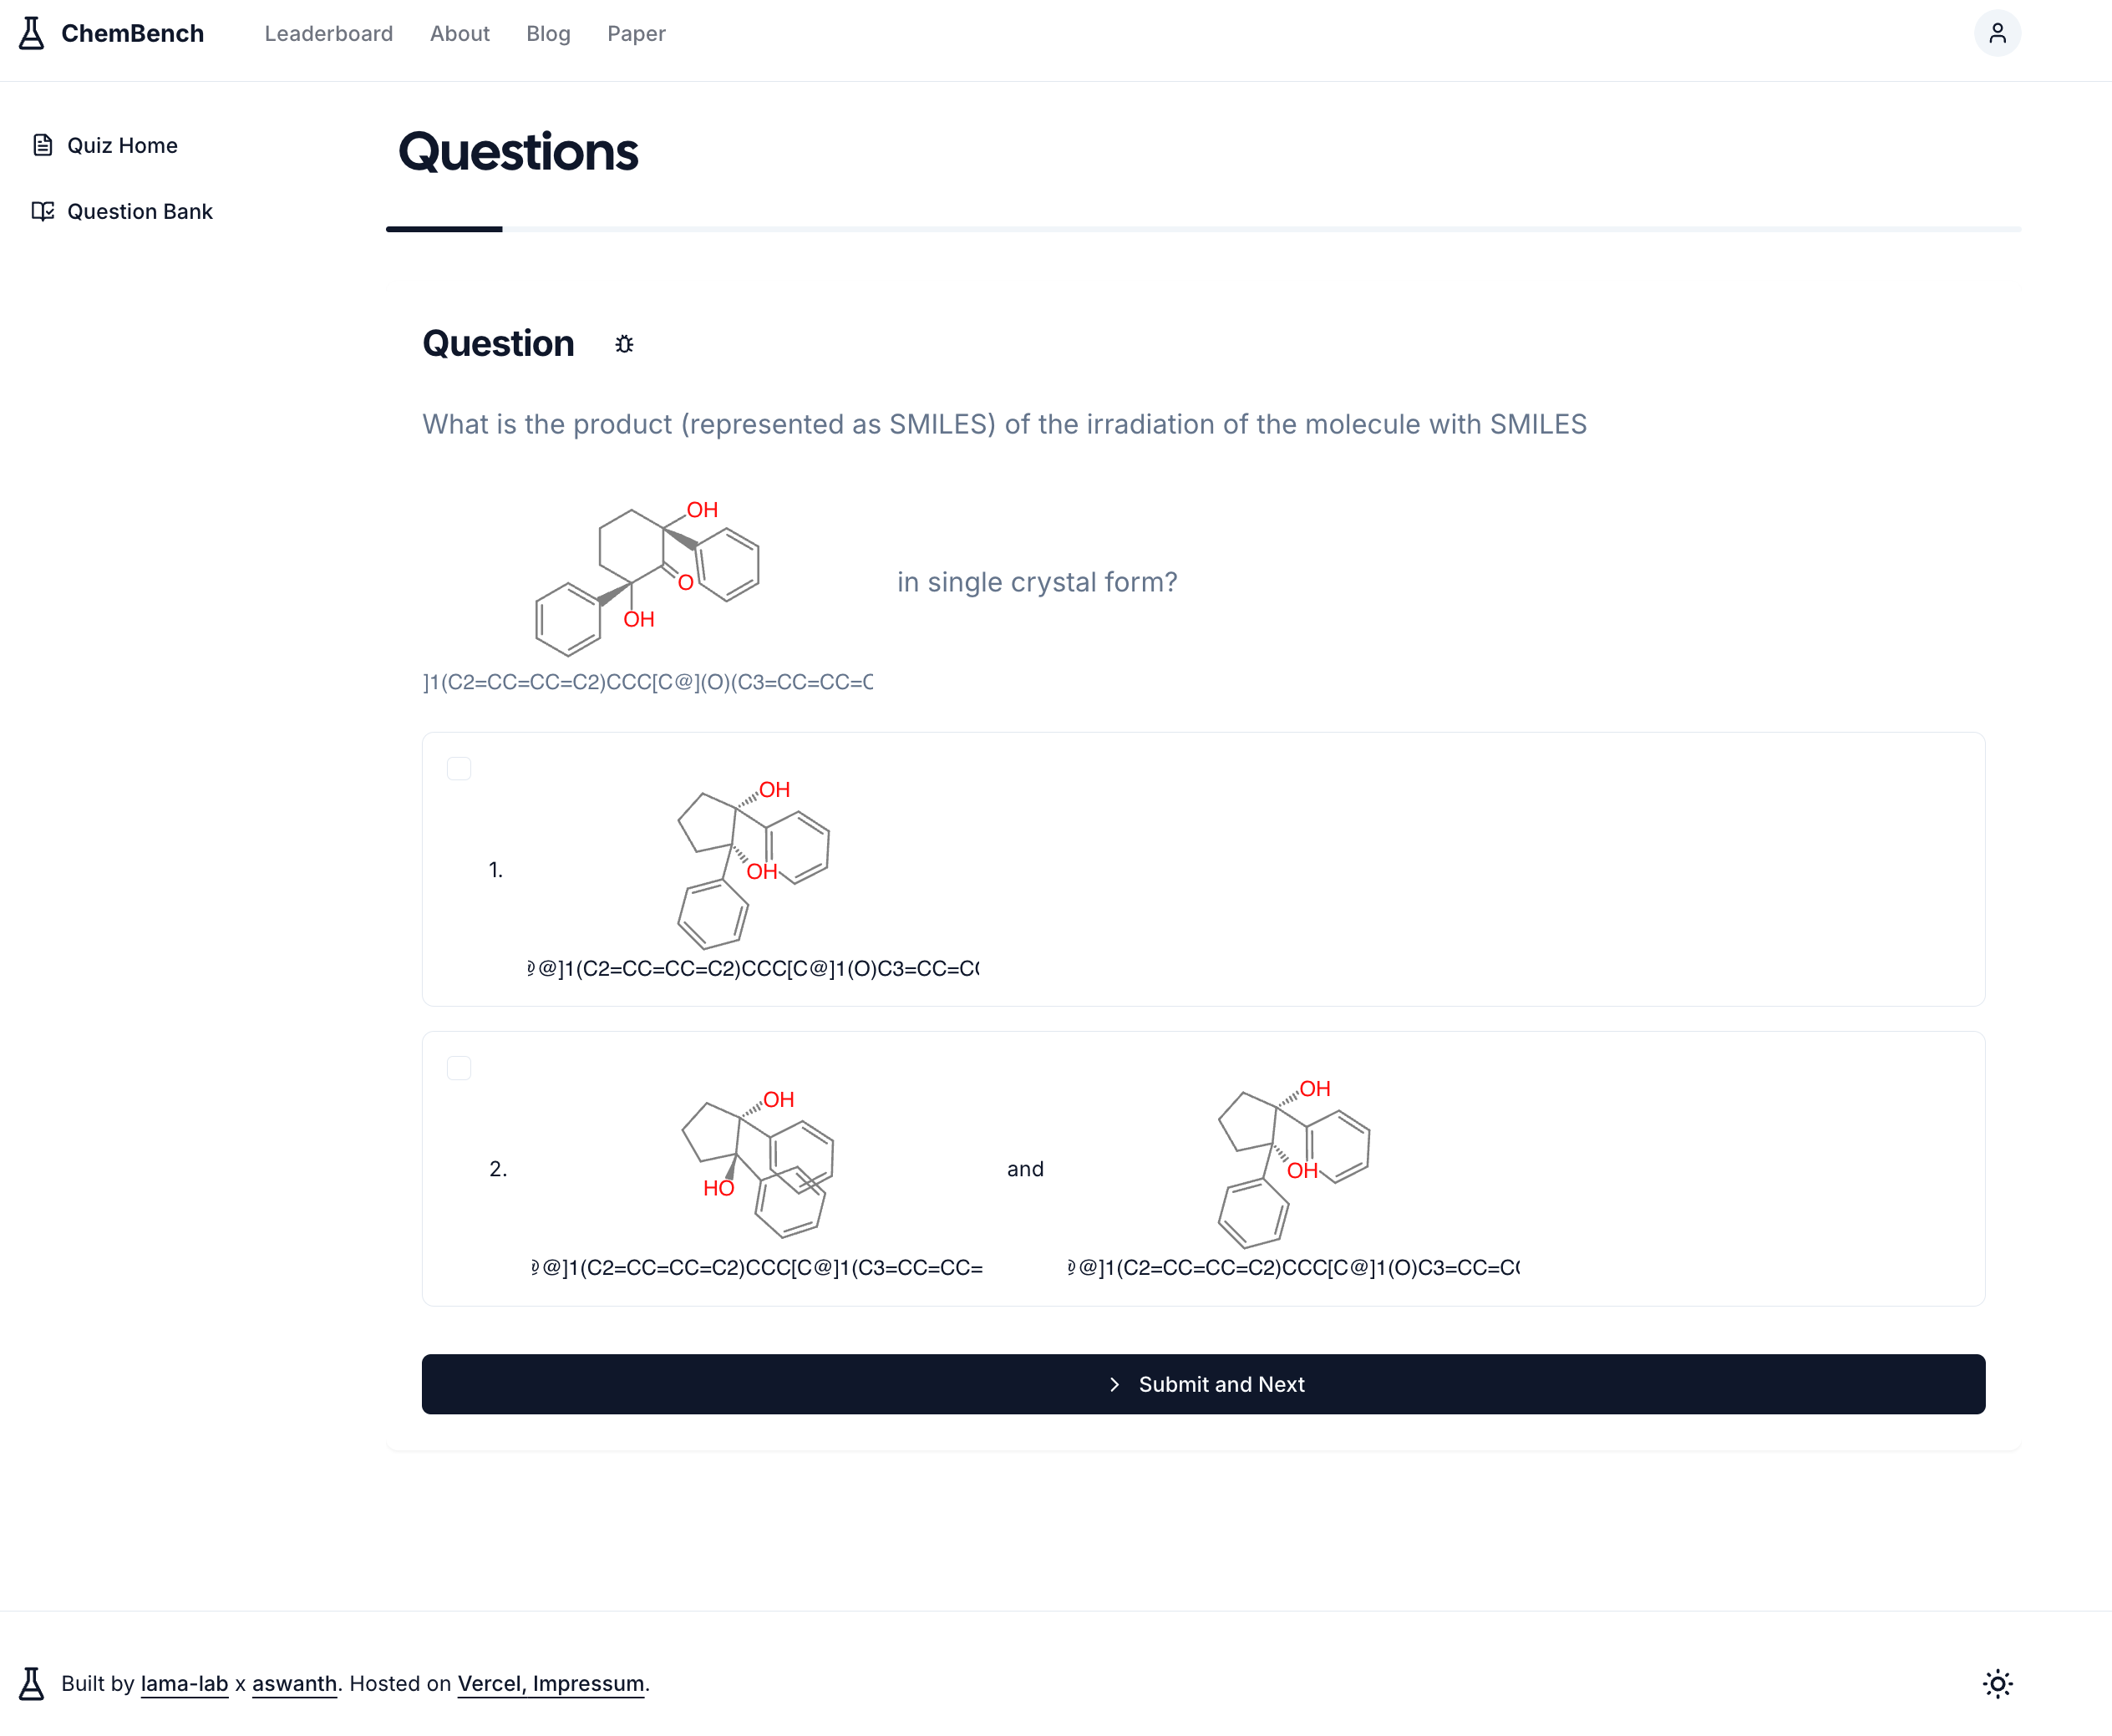
\includegraphics[width=\textwidth]{figures/screenshot_b.png}
    }
    \caption{\textbf{Examples of how questions were shown to the human participants.}}
    \label{fig:screenshots}
\end{figure}

\paragraph{Statistics}
\Cref{fig:human_score_distribution} shows the distribution of scores our human scorers achieved.

\begin{figure}[htb]
    \centering
    \includegraphics{figures/human_score_distribution.pdf}
    \script{plot_human_score_distribution.py}
    \caption{\textbf{Distribution of human scores.} The histogram and kernel density estimates show the fraction of questions answered correctly by the human volunteers.
    Since the best possible score for each question is one and the worst possible score is zero, the values on this plot are between zero and one. A score of one would mean that a volunteer answered all questions correctly. A score of zero would mean that no question was answered correctly.
    We find that the scores for the questions that the human volunteers answered with tools are generally lower than the scores for the questions that the human volunteers answered without tools.
    }
    \label{fig:human_score_distribution}
\end{figure}

We also recorded the time humans took to answer the questions. This time is the time from the question being displayed to the human to the human submitting the answer.

\begin{figure}[htb]
    \centering
    \includegraphics{figures/human_timing.pdf}
    \script{analyze_human_data.py}
    \caption{\textbf{Time taken by human scorers to answer questions vs.\ correctness of their answers.} From the plot, it is clear that there is no clear dependence of the correctness of the answers on the time taken by the human scorers to answer the questions. However, we see that human scorers typically took longer to correctly answer questions with tool use.}
    \label{fig:human_timing}
\end{figure}

Additionally, we prompted users to provide additional information about their experience in chemistry.
While we recorded fine-grained information, e.g., their specialization, we focused on the number of years since the first university-level chemistry course.
\Cref{fig:experience_vs_correctness} shows that the experience of the human scorers was weakly correlated with the correctness of their answers (\Cref{fig:experience_vs_correctness}, Spearman's \(\rho \approx \variable{output/spearman_experience_score.txt}\), and \(p \approx \variable{output/spearman_experience_score_p.txt}\)).

\begin{figure}[htb]
    \centering
    \includegraphics{figures/experience_vs_correctness.pdf}
    \script{analyze_human_data.py}
    \caption{\textbf{Experience of human  scorers vs.\ correctness of their answers.} The experience (in the number of years since the first university-level chemistry course) of the human scorers wasp correlated with the correctness of their answers.}
    \label{fig:experience_vs_correctness}
\end{figure}

\paragraph{Tool use}
In our study, humans were allowed to use tools for answering some questions.
They could also report what tools they used for answering questions. As \Cref{fig:tool_use} shows, the most commonly tool was some form of web search (which, according to the freetext responses, often was a multi-step process).

\begin{figure}
    \centering
    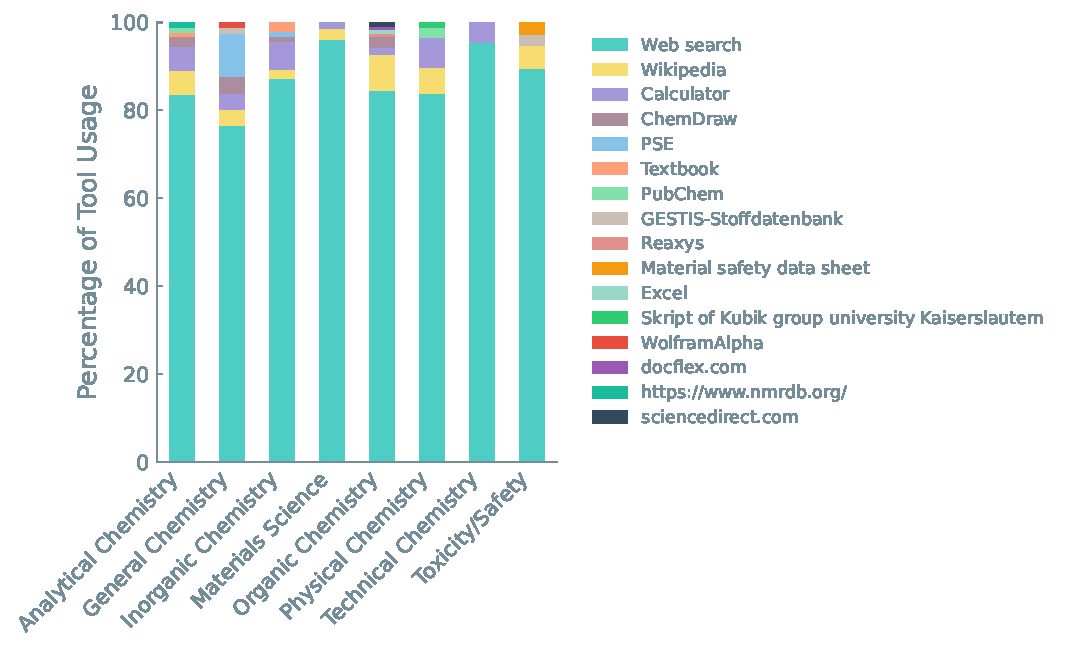
\includegraphics[width=\textwidth]{figures/human_tool_usage_by_topic.pdf}
    \script{human_tool_usage.py}
    \caption{\textbf{Tool usage by human scorers.} The plot shows the most commonly used tools by human participants.}
    \label{fig:tool_use}
\end{figure}

\clearpage
\subsection{Confidence estimates} \label{sec:confidence_estimates}

Since it is important to understand if models can provide an indication of whether their answer might likely be incorrect, we prompted some of our top performing \glspl{llm} to return the confidence in providing a correct answer on an ordinal scale.
This is similar to the verbalized confidence scores reported by \textcite{xiong2023llms}.
We find that the models show different distributions of confidence scores, which, for some, are skewed to the extremes.

In addition, we also analyzed the confidence estimated via the log probabilities of the answer tokens. This probability of a token given the context is not necessarily the same as the confidence in the correctness of the answer. However, it is still often used as a proxy.

Our analysis of both log probabilities and prompting confidence reveals distinct calibration behaviors across different language models.
\GPTFourO demonstrates an overconfident tendency, often assigning high probabilities even to incorrect answers.
However, when \GPTFourO displays high confidence, it accurately predicts correct answers approximately \SI{80}{\percent} of the time. In contrast, \LlamaThreeOneEightBInstruct confidence distribution is more evenly spread, with a majority of predictions centered around 0.5. High-confidence predictions from \LlamaThreeOneEightBInstruct are less frequent compared to \GPTFourO, and unlike \GPTFourO, high confidence does not necessarily correlate with a higher chance of correct answers.

\begin{figure}[htb]
    \centering
    \includegraphics[width=\textwidth]{figures/log_probs_calibration_plot_overall_filtered.pdf}
    \caption{\textbf{Reliability diagram of histogram of logit-based confidence estimates.} For this analysis we obtained the linear probability from the logprobs of the models. Only logprobs of the tokens corresponding to the answers were considered. Linear proabability was computed by taking exponential of logprobs (for sequences with multiple tokens, values were multiplied).  The plot shows the average predicted probability and the fraction of correct answers for each bin of linear probabilities. The ideal scenario is a diagonal line, indicating perfect calibration where the model's confidence aligns perfectly with the actual correctness. The \gls{ece} value quantifies the overall calibration performance, with a lower \gls{ece} indicating better calibration.}
    \label{fig:confidence_score_distributions}
    \script{plot_logprobs.py}
\end{figure}

\clearpage
\subsection{Impact of sampling temperature}
We also investigated the impact of sampling temperature (i.e. temperature 0 means always sampling the most likely token, higher temperatures introduce some randomness in the generation process) on the performance of the models. \Cref{fig:temperature_impact} shows that, generally, the performance of models tends to decrease with increasing temperature.

\begin{figure}[!h]
    \centering
    \includegraphics{figures/swarm_plot_combined.pdf}
    \caption{\textbf{Impact of sampling temperature on the performance of the models.} The plot shows the performance of the models at zero temperature (i.e., greedy decoding) and temperature of one. The performance is measured in terms of the fraction of questions answered correctly.}
    \label{fig:temperature_impact}
    \script{plot_temperature_diffs.py}
\end{figure}





\clearpage
\subsection{Leaderboard}
Our leaderboard is based on the tool chain developed for Matbench.\autocite{Dunn_2020}
Briefly, the \chembench pipeline produces standardized files in \texttt{json} format that contributors can add via pull requests to the \chembench repository.
The Markdown tables and interactive plots are automatically generated and updated on the \chembench website. The leaderboard is available at \url{https://lamalab-org.github.io/chem-bench/leaderboard/}.

\clearpage

\printnoidxglossary[type=\acronymtype, nonumberlist]  % https://github.com/tectonic-typesetting/tectonic/issues/704

\clearpage
\printbibliography[heading=subbibintoc]
\end{refsection}
\end{document}
